% paper_ViGATs_JIT_Revised_Clean.tex
% Formatted for Journal of Information and Telecommunication (JIT)
% Taylor & Francis -- Interact layout + APA reference style (Revised Clean Manuscript)

\documentclass[]{interact}

\usepackage{epstopdf}
\usepackage[caption=false]{subfig}
\usepackage[sort]{natbib}
\bibpunct[, ]{(}{)}{;}{a}{,}{,}
\renewcommand\bibfont{\fontsize{10}{12}\selectfont}

\theoremstyle{plain}
\newtheorem{theorem}{Theorem}[section]
\newtheorem{lemma}[theorem]{Lemma}
\newtheorem{corollary}[theorem]{Corollary}
\newtheorem{proposition}[theorem]{Proposition}

\theoremstyle{definition}
\newtheorem{definition}[theorem]{Definition}
\newtheorem{example}[theorem]{Example}

\theoremstyle{remark}
\newtheorem{remark}{Remark}
\newtheorem{notation}{Notation}

% Additional packages
\usepackage{multirow}
\usepackage{float}
\usepackage{algorithm}
\usepackage{algpseudocode}
\renewcommand{\algorithmiccomment}[1]{\hfill\textcolor{black!60}{\textit{// #1}}}
\usepackage{url}
\def\UrlBreaks{\do\/\do-}
\usepackage{hyperref}
\usepackage{xcolor}

\definecolor{bestblue}{RGB}{0,100,200}
\definecolor{secondorange}{RGB}{230,150,0}
\definecolor{bestgreen}{RGB}{0,128,80}
\newcommand{\bestresult}[1]{\textcolor{bestgreen}{\textbf{#1}}}
\newcommand{\secondresult}[1]{\textcolor{secondorange}{#1}}

\hypersetup{
  unicode=true,
  pdfencoding=auto,
  breaklinks=true,
  colorlinks=true,
  linkcolor=blue,
  citecolor=blue,
  urlcolor=blue
}

\raggedbottom
\begin{document}

\articletype{RESEARCH ARTICLE}

\title{ViGATs: Vision Graph Attention Networks for Enhanced Plant Leaf Disease Classification}

\author{
\name{Anonymous Authors for Double-Blind Review}
\affil{Manuscript submitted to Journal of Information and Telecommunication (JIT)}
}

\maketitle

\begin{abstract}
Automated plant disease diagnosis is crucial for food security and precision agriculture, yet it faces substantial challenges from irregularly scattered lesions, diverse symptoms, and intricate natural field backgrounds. While Vision Graph Neural Networks (Vision GNNs) mitigate the rigid local receptive fields of conventional Convolutional Neural Networks (CNNs), their standard Max-Relative graph convolution (MRConv) assigns hard, unweighted extreme responses across channels. In this paper, we propose ViGATs (Vision Graph Attention Networks), integrating a novel Edge-Difference Multi-Head Graph Attention Convolution (GATConv) module with grouped linear projections to learn adaptive, context-sensitive attention weights among dynamic image patch neighbors. Operating under a rigorous \emph{train-from-scratch paradigm at low input resolution ($64 \times 64$)}, ViGATs is comprehensively evaluated using 5-fold stratified cross-validation across four diverse plant disease benchmarks (PlantVillage, Maize Disease, Rice Leaf V2, and the multicrop in-the-wild PlantRaw), the standard Tiny ImageNet dataset, and an unseen aerial drone cross-domain transfer benchmark (IIITDMJ). ViGATs establishes superior performance with an average classification accuracy of $96.09\%$ across all plant benchmarks, notably achieving $86.12\%$ on complex in-field PlantRaw images and outperforming modern CNNs, Vision Transformers, and State Space Models. Requiring only 4.67M parameters and 1.13 GFLOPs, ViGATs provides a balanced and efficient architecture for edge-AI agricultural diagnostic systems.
\end{abstract}

\begin{keywords}
Graph Attention Networks; Vision GNN; Plant Disease Classification; Stratified Cross-Validation; Cross-Domain Transfer; Smart Agriculture
\end{keywords}


\section{Introduction}
\label{sec:introduction}

Plant foliar diseases account for an estimated 20\% to 40\% loss in global crop production annually \citep{savary2019global}, directly threatening food security and agricultural sustainability. Early, automated, and accurate detection of foliar pathologies from digital imagery is a cornerstone of smart agriculture and intelligent precision farming. Deep learning has fundamentally advanced automated disease diagnosis through three principal visual representation paradigms:

\begin{enumerate}
    \item \textit{Convolutional Neural Networks (CNNs):} Exploit local spatial correlations over rigid, rectangular pixel grids \citep{he2016deep, liu2022convnext}.
    \item \textit{Vision Transformers (ViTs):} Utilize multi-head self-attention mechanisms to model global dependencies across sequence patch tokens \citep{dosovitskiy2020image, liu2021swin}.
    \item \textit{Vision Graph Neural Networks (Vision GNNs):} Transform an image into an unstructured, dynamic feature-space graph, flexibly linking scattered and non-contiguous symptoms regardless of spatial distance \citep{han2022vision} (as conceptualized in Figure~\ref{fig:img2graph}).
\end{enumerate}

\begin{figure}[H]
\centering
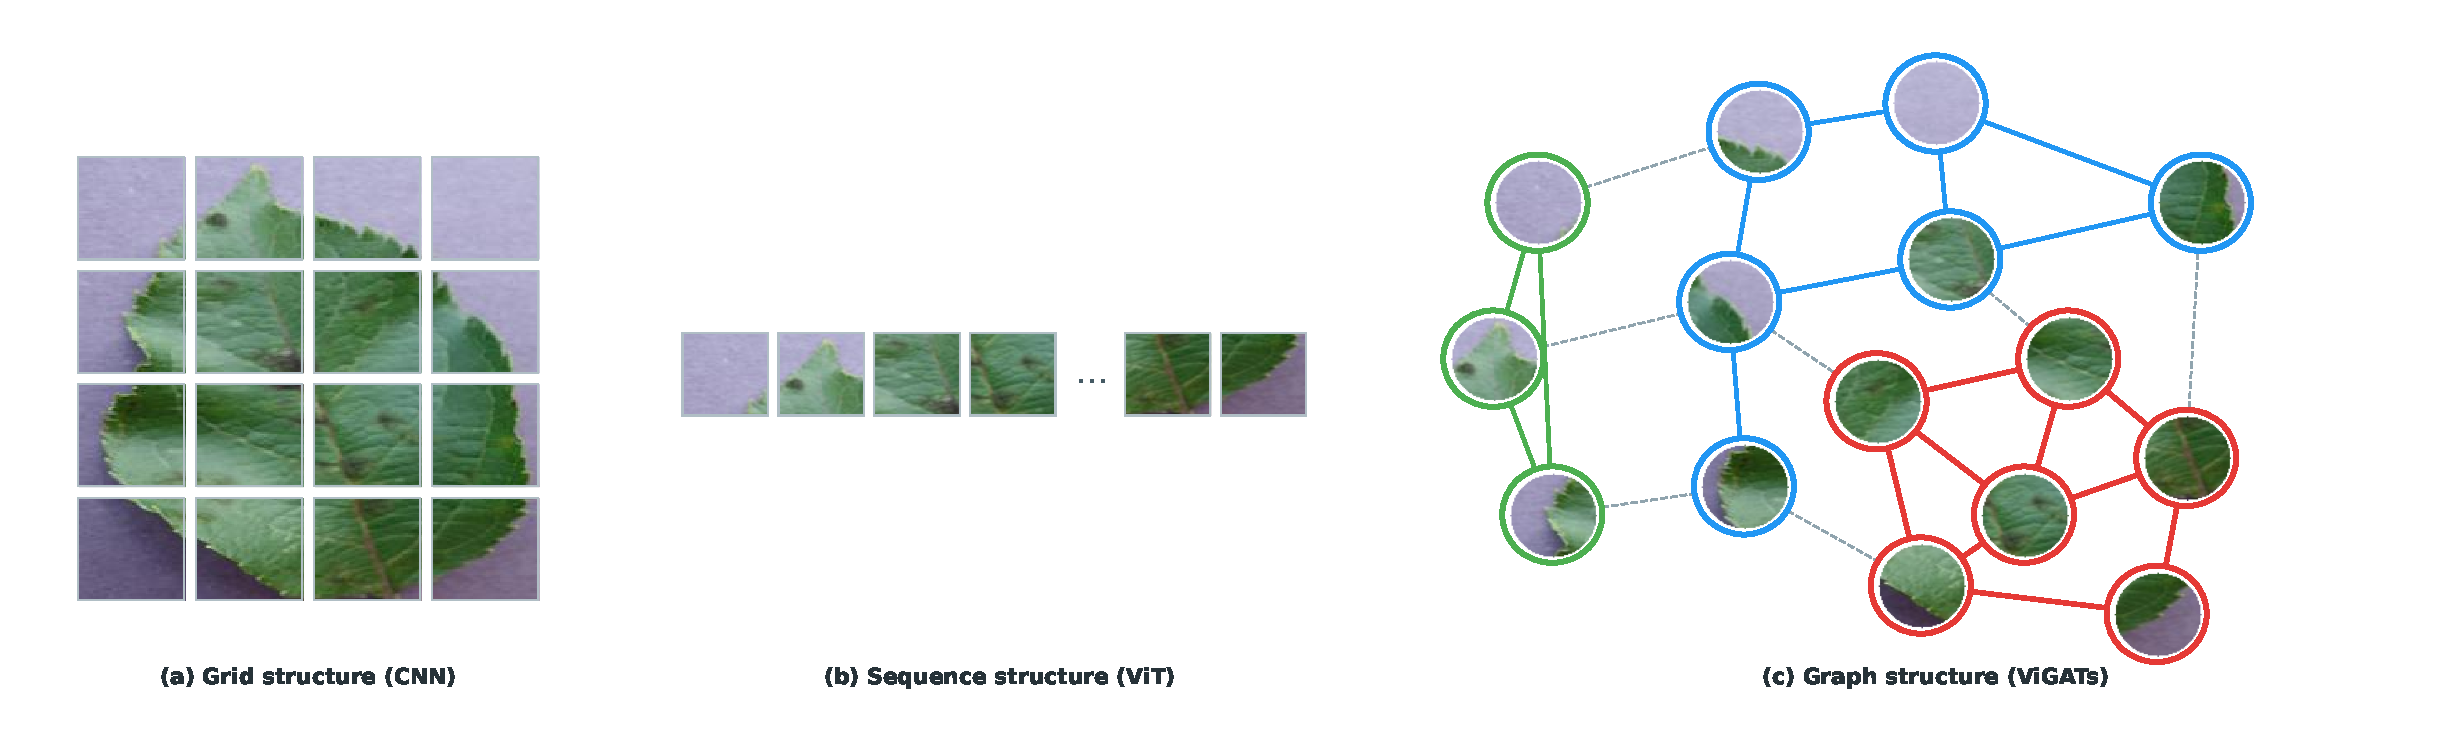
\includegraphics[width=\textwidth]{figures/Figure_01_image_to_graph.pdf}
\caption{Comparison of three visual representation paradigms: (a) regular grid (CNNs); (b) token sequence (ViTs); and (c) dynamic feature-space graph (ViGATs).}
\label{fig:img2graph}
\end{figure}

Despite notable achievements, existing architectures present fundamental limitations when deployed in practical agricultural scenarios. Standard CNNs are constrained by fixed, local receptive fields, rendering them suboptimal for capturing non-contiguous lesions scattered across irregular leaf surfaces. Vision Transformers impose quadratic computational complexity and frequently suffer from severe over-fitting when trained from scratch on compact domain-specific datasets. Concurrently, original Vision GNNs rely on Max-Relative Convolution (MRConv) \citep{li2019deepgcns, han2022vision}, which applies a channel-wise hard maximum operation over neighbor differences. Although MRConv selectively captures peak responses, it treats neighbor contributions rigidly without learning soft contextual importance, making it vulnerable to complex field noise and fluctuating illumination.

To address these challenges, we introduce ViGATs (Vision Graph Attention Networks). Diverging from common approaches that rely on large-scale pre-trained weights at high resolutions ($224 \times 224$), we formulate a challenging yet practical benchmark: \emph{training from scratch at a low input resolution of $64 \times 64$}. This setting faithfully mirrors the hardware, memory, and bandwidth constraints of real-world edge IoT sensor nodes and unmanned aerial vehicles (UAVs). ViGATs re-engineers the graph convolution layer by introducing a specialized GATConv module. By computing multi-head attention coefficients ($H=4$) over edge differences $(\mathbf{x}_j - \mathbf{x}_i)$ via efficient grouped projections, ViGATs dynamically prioritizes pathological lesion boundaries while effectively suppressing background noise.

The primary contributions of this work are summarized as follows:
\begin{itemize}
    \item \textit{Edge-Difference GATConv Module:} We design a multi-head edge-difference graph attention convolution combined with node-level grouped projections, resolving both the static attention bottleneck and the excessive computational overhead of GAT and GATv2.
    \item \textit{Compact Edge-AI Architecture:} ViGATs achieves a highly optimized footprint with only 4.67M parameters, 1.13 GFLOPs, and 129.8 MB peak VRAM, providing an optimal trade-off for resource-constrained edge computing.
    \item \textit{Leakage-Free Multi-Dataset Benchmarking:} Through a strict 5-fold stratified cross-validation protocol, ViGATs consistently outperforms CNN, ViT, and SSM baselines across four plant disease datasets (PlantVillage, Maize Disease, Rice Leaf V2, PlantRaw), Tiny ImageNet, and an unseen aerial drone domain transfer scenario (IIITDMJ).
    \item \textit{Visual Explainability \& Diagnostic Insight:} We demonstrate the model's capability to capture non-local pathological associations through t-SNE manifold projections and attention heatmaps.
\end{itemize}

\section{Related Work}
\label{sec:related-work}

\subsection{CNN-Based Plant Disease Diagnosis}
Deep convolutional networks have long dominated automated plant disease recognition \citep{mohanty2016using}. Widely adopted architectures including VGG \citep{ferentinos2018deep}, ResNet \citep{he2016deep, sethy2020deep, singh2024comprehensive}, EfficientNet \citep{tan2019efficientnet}, and MobileNet \citep{chen2021identification, too2019comparative} have achieved classification accuracies surpassing 97\% on laboratory benchmarks, even under resource-constrained conditions \citep{batool2025compact}. Nevertheless, standard CNNs remain fundamentally constrained by the inductive bias of localized grid convolutions \citep{lecun1998gradient}, creating difficulties when aggregating spatially disconnected, fine-grained lesion symptoms under natural field conditions. Furthermore, most CNN approaches depend heavily on ImageNet pre-trained representations.

\subsection{Vision Transformers}
Vision Transformers (ViTs) \citep{dosovitskiy2020image} overcome local spatial limitations by employing global self-attention across image patch tokens. Recent variants such as DeiT \citep{touvron2021training}, Swin Transformer \citep{liu2021swin}, and hybrid CNN-ViT architectures \citep{yu2025stcfi} have improved efficiency and multi-scale feature extraction. However, ViTs require massive training corpora and lack spatial inductive biases, making them prone to severe optimization instability and over-fitting when trained from scratch on agricultural datasets at low resolutions \citep{borhani2022deep}.

\subsection{Vision Graph Neural Networks and Graph Attention}
Graph Neural Networks (GNNs) formulate images as unstructured, dynamic feature graphs \citep{scarselli2009graph, wu2020comprehensive, zhou2020graph, han2022vision}. Recently, hybrid CNN-GNN frameworks \citep{singla2025denseswingnnnet, surekha2026adjleafgnn} and sparse attention variants such as MobileViG \citep{munir2023mobilevig} and AttentionViG \citep{gedik2025attentionvig} have emerged. Concurrently, Graph Attention Networks (GAT \citep{velickovic2018graph} and GATv2 \citep{brody2022gat}) have demonstrated marked advantages in learning adaptive neighborhood importance. This study bridges the gap by directly integrating an edge-difference multi-head attention mechanism into the isotropic Vision GNN framework, creating an efficient and robust architecture (ViGATs) optimized for botanical pathology diagnosis.


\section{Proposed Method: ViGATs}
\label{sec:methodology}

\subsection{Architecture Overview and Design Rationale}
ViGATs follows the isotropic visual graph framework established by ViG \citep{han2022vision}: a convolutional stem extracts early visual features, an image-to-graph module constructs a dynamic $K$-Nearest Neighbor ($K$-NN) graph in metric feature space, and repeated Grapher--FFN blocks iteratively update node representations. Our core architectural innovation is replacing the standard MRConv with the proposed GATConv module (illustrated in Figure~\ref{fig:architecture}), enabling adaptive, content-aware attention across neighboring patches.

\begin{figure}[H]
\centering
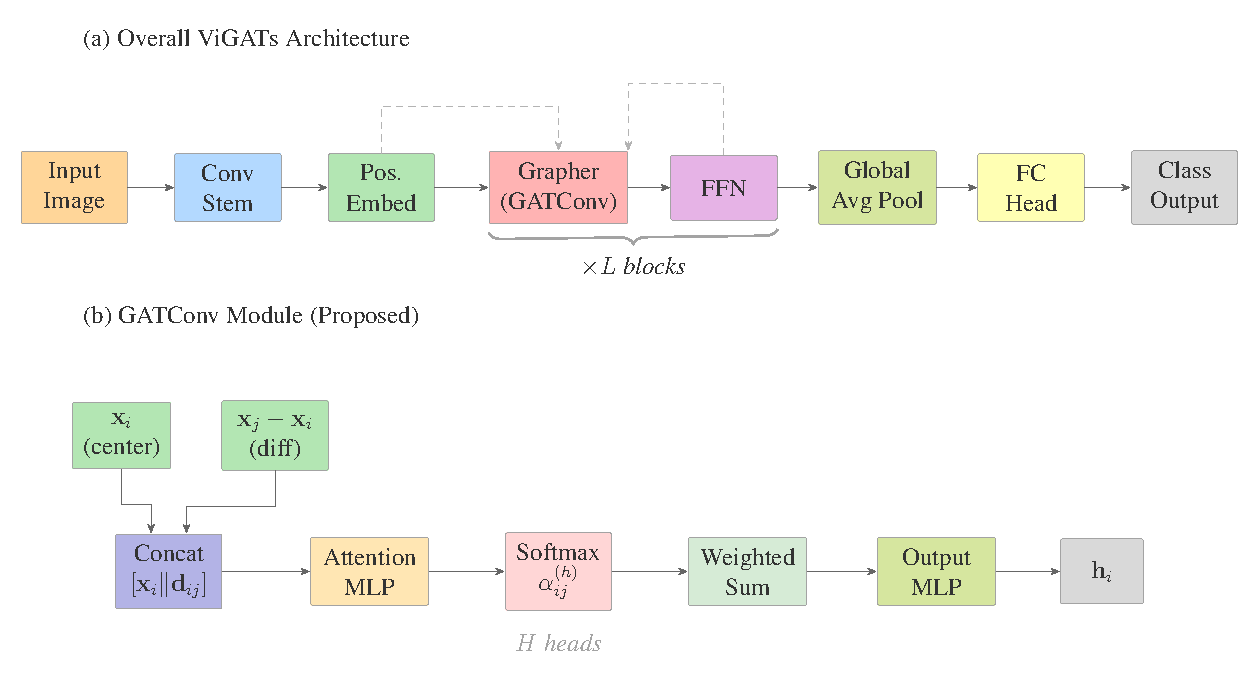
\includegraphics[width=\textwidth]{figures/Figure_02_architecture.pdf}
\caption{Overview of the ViGATs architecture: (a) the complete processing pipeline; and (b) the proposed GATConv module aggregating neighbor differences using multi-head edge attention.}
\label{fig:architecture}
\end{figure}

\subsection{Image-to-Graph Transformation}
\label{sec:image_to_graph}

The overall pipeline transforming an input image into a dynamic graph within ViGATs is depicted in Figure~\ref{fig:vigats_framework}.

\begin{figure}[H]
\centering
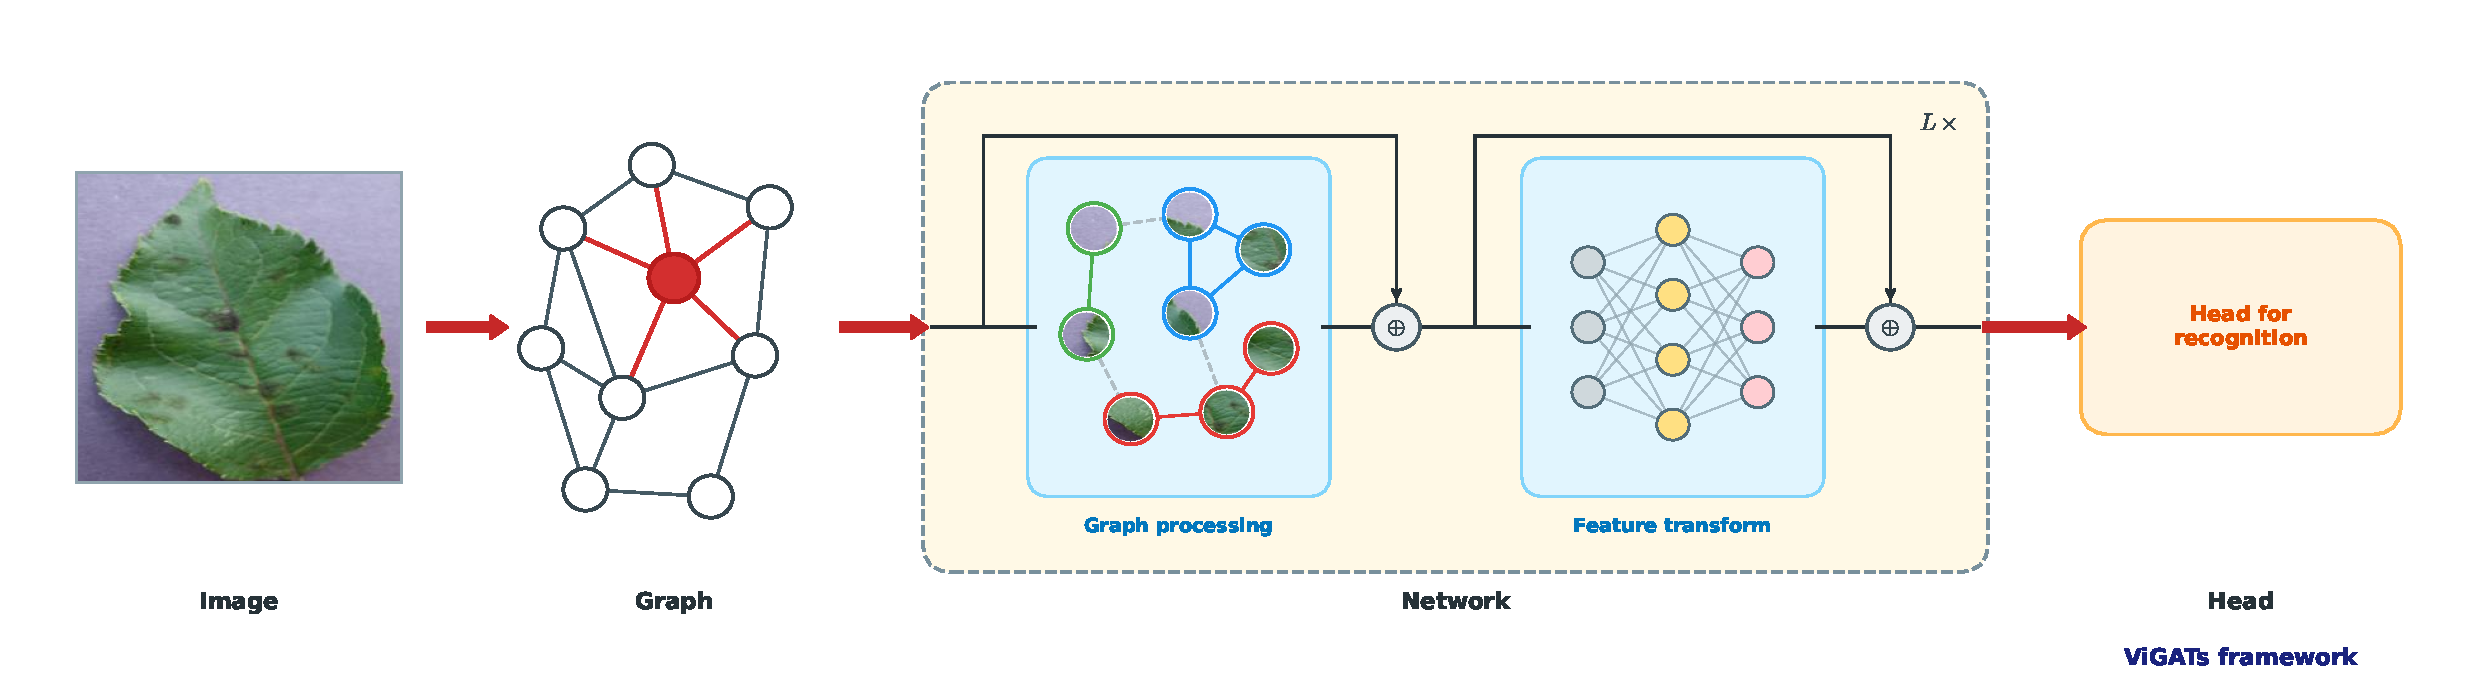
\includegraphics[width=\textwidth]{figures/Figure_03_vigats_framework.pdf}
\caption{ViGATs processing framework from an input image to a dynamic graph, repeated Grapher--FFN blocks, global pooling, and the final classification.}
\label{fig:vigats_framework}
\end{figure}

Given an input RGB image $\mathbf{I} \in \mathbb{R}^{3 \times H \times W}$, a convolutional stem consisting of three $3 \times 3$ convolutional layers with Batch Normalization (BN) \citep{ioffe2015batch} and GELU non-linearities \citep{hendrycks2016gaussian} downsamples the spatial dimensions by a factor of 4, producing feature map $\mathbf{X} \in \mathbb{R}^{C \times H' \times W'}$ where $H' = H/4, W' = W/4$:
\begin{equation}
\text{Stem}(\mathbf{I}) = \text{Conv}_{3\times3}^{(C \rightarrow C)}\Big(\text{GELU}\big(\text{BN}(\text{Conv}_{3\times3, s=2}^{(C/2 \rightarrow C)}(\text{GELU}(\text{BN}(\text{Conv}_{3\times3, s=2}^{(3 \rightarrow C/2)}(\mathbf{I})))))\big)\Big).
\end{equation}
Each spatial grid coordinate $(u, v)$ is treated as an individual node $i$, resulting in $N = H' \times W'$ total nodes $\mathbf{x}_i \in \mathbb{R}^C$. A learnable position encoding tensor $\mathbf{P} \in \mathbb{R}^{1 \times C \times H' \times W'}$ is added to preserve 2D spatial context:
\begin{equation}
\mathbf{X}^{(0)} = \mathbf{X} + \mathbf{P}.
\end{equation}

\subsection{Dynamic $K$-NN Graph Construction}
\label{sec:dynamic_knn}

Semantic distance between any pair of node features $(\mathbf{x}_i, \mathbf{x}_j)$ is measured using normalized $L_2$ Euclidean distance \citep{han2022vision}:
\begin{equation}
d(\mathbf{x}_i, \mathbf{x}_j) = \|\hat{\mathbf{x}}_i - \hat{\mathbf{x}}_j\|_2^2, \qquad \text{where } \hat{\mathbf{x}}_i = \frac{\mathbf{x}_i}{\|\mathbf{x}_i\|_2}.
\end{equation}
For each central node $i$, its local neighborhood $\mathcal{N}_K(i)$ is dynamically constructed by selecting the $K$ nearest neighbors in feature space:
\begin{equation}
\mathcal{N}_K(i) = \arg\min_{j \in \{1, \dots, N\} \setminus \{i\}}^{(K)} d(\mathbf{x}_i, \mathbf{x}_j).
\end{equation}
The graph topology $\mathcal{G}^{(l)} = (\mathcal{V}, \mathcal{E}^{(l)})$ is dynamically recomputed at the entrance of each Grapher block.

\subsection{Max-Relative Graph Convolution (MRConv Baseline)}
\label{sec:mrconv_baseline}

In the original ViG \citep{han2022vision}, neighborhood aggregation is conducted via MRConv:
\begin{equation}
\mathbf{m}_i = \max_{j \in \mathcal{N}_K(i)} (\mathbf{x}_j - \mathbf{x}_i), \qquad \forall i \in \{1, \dots, N\},
\end{equation}
\begin{equation}
\mathbf{h}_i = \text{MLP}\big([\mathbf{x}_i \parallel \mathbf{m}_i]\big).
\end{equation}
While the channel-wise maximum retains peak feature activations, it applies a rigid selection policy that discards the nuanced relative semantic contributions of other neighboring patches, making the model sensitive to background clutter.

\subsection{Edge-Difference Multi-Head Graph Attention Convolution (Proposed GATConv)}
\label{sec:gatconv}

To resolve the limitations of MRConv, we propose the GATConv module. Drawing on the foundational principles of GAT \citep{velickovic2018graph} and dynamic GATv2 \citep{brody2022gat}, GATConv is specifically engineered for visual representations by computing adaptive multi-head attention weights directly on edge-difference vectors $(\mathbf{x}_j - \mathbf{x}_i)$ coupled with high-throughput grouped projections.

The message passing procedure within GATConv for each node $i$ and neighbor $j \in \mathcal{N}_K(i)$ unfolds in four systematic steps:

\textit{Step 1: Neighbor Edge Difference.}
\begin{equation}
\mathbf{d}_{ij} = \mathbf{x}_j - \mathbf{x}_i \in \mathbb{R}^{C}, \qquad \forall j \in \mathcal{N}_K(i).
\label{eq:diff}
\end{equation}

\textit{Step 2: Multi-Head Attention Coefficients.} A linear projection $\mathbf{W}_1 = [\mathbf{W}_{1a} \mid \mathbf{W}_{1b}]$ maps node and edge features into a latent space $D = H \cdot d_k$:
\begin{equation}
\mathbf{g}_{ij} = \sigma_{\text{LR}}\!\Big(\mathbf{W}_{1a}\mathbf{x}_i + \mathbf{W}_{1b}\mathbf{d}_{ij} + \mathbf{b}_1\Big) \in \mathbb{R}^{D}.
\label{eq:attn_hidden}
\end{equation}
The latent vector $\mathbf{g}_{ij}$ is partitioned across $H$ attention heads. Each head $h$ evaluates its unnormalized attention score via grouped linear projection $\mathbf{w}_2^{(h)}$, followed by Softmax normalization:
\begin{equation}
e_{ij}^{(h)} = {\mathbf{w}_2^{(h)}}^\top \mathbf{g}_{ij}^{(h)} + b_2^{(h)}, \qquad h = 1, \dots, H,
\label{eq:attn_logit}
\end{equation}
\begin{equation}
\alpha_{ij}^{(h)} = \frac{\exp\!\big(e_{ij}^{(h)}\big)}{\sum_{k \in \mathcal{N}_K(i)} \exp\!\big(e_{ik}^{(h)}\big)}.
\label{eq:softmax}
\end{equation}

\textit{Step 3: Multi-Head Weighted Aggregation.} The partitioned difference features $\mathbf{d}_{ij}^{(h)}$ are aggregated across all neighbors according to normalized attention coefficients:
\begin{equation}
\mathbf{m}_i = \bigg\|_{h=1}^{H} \sum_{j \in \mathcal{N}_K(i)} \alpha_{ij}^{(h)} \cdot \mathbf{d}_{ij}^{(h)} \in \mathbb{R}^{C}.
\label{eq:agg}
\end{equation}

\textit{Step 4: Representation Update.} Node representations are updated via residual concatenation and grouped $1 \times 1$ linear projection:
\begin{equation}
\mathbf{h}_i = \text{GELU}\!\Big(\text{BN}\!\big(\mathbf{W}_{\text{out}}[\mathbf{x}_i \parallel \mathbf{m}_i] + \mathbf{b}_{\text{out}}\big)\Big).
\label{eq:output}
\end{equation}
Algorithm~\ref{alg:gatconv} details the complete computation workflow.

\begin{algorithm}[H]
\caption{Message Passing and Attention Computation in GATConv}
\label{alg:gatconv}
\begin{algorithmic}[1]
\Require Node feature matrix $\mathbf{X} \in \mathbb{R}^{C \times N}$, dynamic $K$-NN neighborhood $\mathcal{N}_K$, number of heads $H$, head dimension $d_k$ ($D = H \cdot d_k$).
\Ensure Updated node feature matrix $\mathbf{H} \in \mathbb{R}^{C \times N}$.
\State $\mathbf{P}_{\text{src}} = \mathbf{W}_{1a} \mathbf{X}, \quad \mathbf{P}_{\text{dst}} = \mathbf{W}_{1b} \mathbf{X}$ \Comment{Step 1: Node-level projections ($\mathbb{R}^{D \times N}$)}
\For{each node $i \in \{1, \dots, N\}$ and neighbor $j \in \mathcal{N}_K(i)$}
    \State $\mathbf{d}_{ij} = \mathbf{x}_j - \mathbf{x}_i$ \Comment{Edge difference vector}
    \State $\mathbf{g}_{ij} = \text{LeakyReLU}_{0.2}\big(\mathbf{P}_{\text{src}, i} + \mathbf{P}_{\text{dst}, j} - \mathbf{P}_{\text{dst}, i}\big)$ \Comment{Step 2: Attention logits ($\mathbb{R}^{D}$)}
    \For{each attention head $h \in \{1, \dots, H\}$}
        \State $e_{ij}^{(h)} = {\mathbf{w}_2^{(h)}}^\top \mathbf{g}_{ij}^{(h)} + b_2^{(h)}$ \Comment{Grouped projection ($\text{groups}=H$)}
        \State $\alpha_{ij}^{(h)} = \frac{\exp(e_{ij}^{(h)})}{\sum_{k \in \mathcal{N}_K(i)} \exp(e_{ik}^{(h)})}$ \Comment{Softmax normalization}
    \EndFor
    \State $\mathbf{m}_i = \Big\|_{h=1}^H \sum_{j \in \mathcal{N}_K(i)} \alpha_{ij}^{(h)} \cdot \mathbf{d}_{ij}^{(h)}$ \Comment{Step 3: Multi-head aggregation ($\mathbb{R}^C$)}
    \State $\mathbf{h}_i = \text{GELU}\Big(\text{BN}\big(\mathbf{W}_{\text{out}}[\mathbf{x}_i \parallel \mathbf{m}_i] + \mathbf{b}_{\text{out}}\big)\Big)$ \Comment{Step 4: Output projection ($\mathbb{R}^C$)}
\EndFor
\State \Return $\mathbf{H} = [\mathbf{h}_1, \dots, \mathbf{h}_N]$
\end{algorithmic}
\end{algorithm}

\subsection{Structural Comparison of Graph Operators}
\label{sec:operator_comparison}

We analyze the evolutionary trajectory across four distinct visual graph operators (summarized in Table~\ref{tab:gnn_architectures}):

\textit{MRConv \citep{han2022vision}:} Non-attentive maximum pooling: $\mathbf{m}_i = \max_{j \in \mathcal{N}_K(i)} (\mathbf{x}_j - \mathbf{x}_i)$.

\textit{GAT \citep{velickovic2018graph}:} Static attention scoring $e_{ij}^{(h)} = \sigma_{\text{LR}}\!\Big({\mathbf{a}_{\text{src}}^{(h)}}^\top \mathbf{W}\mathbf{x}_i + {\mathbf{a}_{\text{dst}}^{(h)}}^\top \mathbf{W}\mathbf{x}_j\Big)$, which suffers from rank collapse in dynamic neighborhoods \citep{brody2022gat}.

\textit{GATv2 \citep{brody2022gat}:} Dynamic edge-concatenation attention $e_{ij}^{(h)} = {\mathbf{a}^{(h)}}^\top \sigma_{\text{LR}}\!\Big(\mathbf{W}[\mathbf{x}_i \parallel \mathbf{x}_j]\Big)$, resolving static attention at the expense of high computational complexity (1.81 GFLOPs).

\textit{GATConv (Proposed):} Dynamic edge-difference attention $e_{ij}^{(h)} = {\mathbf{w}_2^{(h)}}^\top \sigma_{\text{LR}}\!\Big(\mathbf{W}_{1a}\mathbf{x}_i + \mathbf{W}_{1b}(\mathbf{x}_j - \mathbf{x}_i) + \mathbf{b}_1\Big)$. GATConv retains the full expressive capacity of dynamic attention while reducing computational cost to 1.13 GFLOPs (a $37.6\%$ savings compared to GATv2).

\begin{table}[H]
\centering
\small
\tbl{Network architecture specifications of evaluated Vision GNN models.}
{\begin{tabular}{lcccc} \toprule
\textbf{Stage / Layer} & \textbf{ViG (Baseline)} & \textbf{ViG+GAT} & \textbf{ViG+GATv2} & ViGATs (Proposed) \\ \midrule
Stem & $\text{Conv} \times 3$ & $\text{Conv} \times 3$ & $\text{Conv} \times 3$ & $\text{Conv} \times 3$ \\
     & $C = 192$ & $C = 192$ & $C = 192$ & $C = 192$ \\ \midrule
Graph & Node $16 \times 16$ & Node $16 \times 16$ & Node $16 \times 16$ & Node $16 \times 16$ \\
      & KNN ($K=7$) & KNN ($K=5$) & KNN ($K=5$) & KNN ($K=5$) \\ \midrule
Graph Operator & MRConv \citep{han2022vision} & GAT \citep{velickovic2018graph} & GATv2 \citep{brody2022gat} & GATConv (Ours) \\
Attention Paradigm & None (Max-Relative) & Static Attention & Dynamic (Edge-Concat) & \textbf{Dynamic (Edge-Diff)} \\
Projection Level & Feature Max & Node-level & Edge-level $[2C \cdot K]$ & \textbf{Node-level $[D+H]$} \\ \midrule
Grapher Blocks & Grapher $\times 8$ & Grapher $\times 8$ & Grapher $\times 8$ & Grapher $\times 8$ \\
               & FFN $\times 8$ & FFN $\times 8$ & FFN $\times 8$ & FFN $\times 8$ \\
               & $C = 192$ & $C = 192,\ H = 4$ & $C = 192,\ H = 4$ & $C = 192,\ H = 4$ \\ \midrule
Head & Pooling \& MLP & Pooling \& MLP & Pooling \& MLP & Pooling \& MLP \\ \midrule
Params & 4.37M & 4.68M & 4.97M & \textbf{4.67M} \\
GFLOPs & 1.05 & 1.82 & 1.81 & \textbf{1.13} \\ \bottomrule
\end{tabular}}
\label{tab:gnn_architectures}
\end{table}

\subsection{Parameter and Computational Complexity Analysis}

Table~\ref{tab:model_complexity} summarizes computational complexity measured on an NVIDIA GeForce RTX 5070 Ti GPU with $64 \times 64$ inputs. ViGATs (38-layer configuration) contains 4.67M parameters, providing an optimal trade-off between feature representation power and physical hardware consumption on edge devices.

\begin{table}[H]
\small
\setlength{\tabcolsep}{3pt}
\tbl{Computational complexity comparison of evaluated models. \textcolor{bestblue}{Blue} = best; \textcolor{secondorange}{orange} = second best.}
{\begin{tabular}{llrrrrr} \toprule
\textbf{Family} & \textbf{Model} & \textbf{Params (M)} & \textbf{Train (M)} & \textbf{GFLOPs} & \textbf{Mem (MB)} & \textbf{FPS} \\ \midrule
\multirow{3}{*}{CNN}
 & ResNet-18 \citep{he2016deep}           & 11.20 & 11.20 & \textcolor{secondorange}{0.15} & \textcolor{bestblue}{68.0}  & \textcolor{bestblue}{439.9} \\
 & ConvNeXt-Tiny \citep{liu2022convnext}  & 27.85 & 27.85 & 0.36 & 169.6 & 218.3 \\
 & EfficientNetV2-S \citep{tan2021efficientnetv2} & 20.23 & 20.23 & 0.24 & \textcolor{secondorange}{88.5} & 66.5 \\ \midrule
\multirow{2}{*}{Transformer}
 & ViT \citep{dosovitskiy2020image}       & 5.62  & 5.62  & 0.95 & 111.8 & \textcolor{secondorange}{410.2} \\
 & Swin-T \citep{liu2021swin}             & 27.55 & 27.55 & 0.24 & 217.5 & 101.9 \\ \midrule
SSM
 & MambaOut-Tiny \citep{yu2024mambaout}   & 24.33 & 24.33 & 0.37 & 197.4 & 168.9 \\ \midrule
\multirow{3}{*}{Lightweight}
 & FastViT-T8 \citep{vasu2023fastvit}     & \textcolor{bestblue}{3.29}  & \textcolor{bestblue}{3.29}  & \textcolor{bestblue}{0.04} & 121.8 & 129.6 \\
 & RepViT-M1 \citep{wang2024repvit}       & 4.74  & 4.74  & 0.07 & 127.5 & 93.1 \\
 & EfficientViT-B1 \citep{cai2023efficientvit} & 7.56 & 7.56 & 0.05 & 137.1 & 64.9 \\ \midrule
\multirow{4}{*}{GNN}
 & ViG \citep{han2022vision}              & \textcolor{secondorange}{4.37}  & \textcolor{secondorange}{4.37}  & 1.05 & 204.6 & 91.4 \\
 & ViG+GAT \citep{velickovic2018graph}    & 4.68  & 4.68  & 1.82 & 112.6 & 73.6 \\
 & ViG+GATv2 \citep{brody2022gat}         & 4.97  & 4.97  & 1.81 & 115.6 & 80.1 \\
 & ViGATs (Proposed)             & 4.67  & 4.67  & 1.13 & 129.8 & 74.0 \\ \bottomrule
\end{tabular}}
\label{tab:model_complexity}
\end{table}

\subsection{Numerical Walkthrough Workflow}
\label{sec:numerical_walkthrough}

Figure~\ref{fig:dataflow_pipeline} illustrates the step-by-step computational workflow of ViGATs on a representative leaf image through five distinct stages: patch partitioning, dynamic $K$-NN graph creation, GATConv edge aggregation, residual updating, and final classification. Concurrently, Table~\ref{tab:vigats_config} summarizes the default hyperparameters.

\begin{figure}[H]
\centering
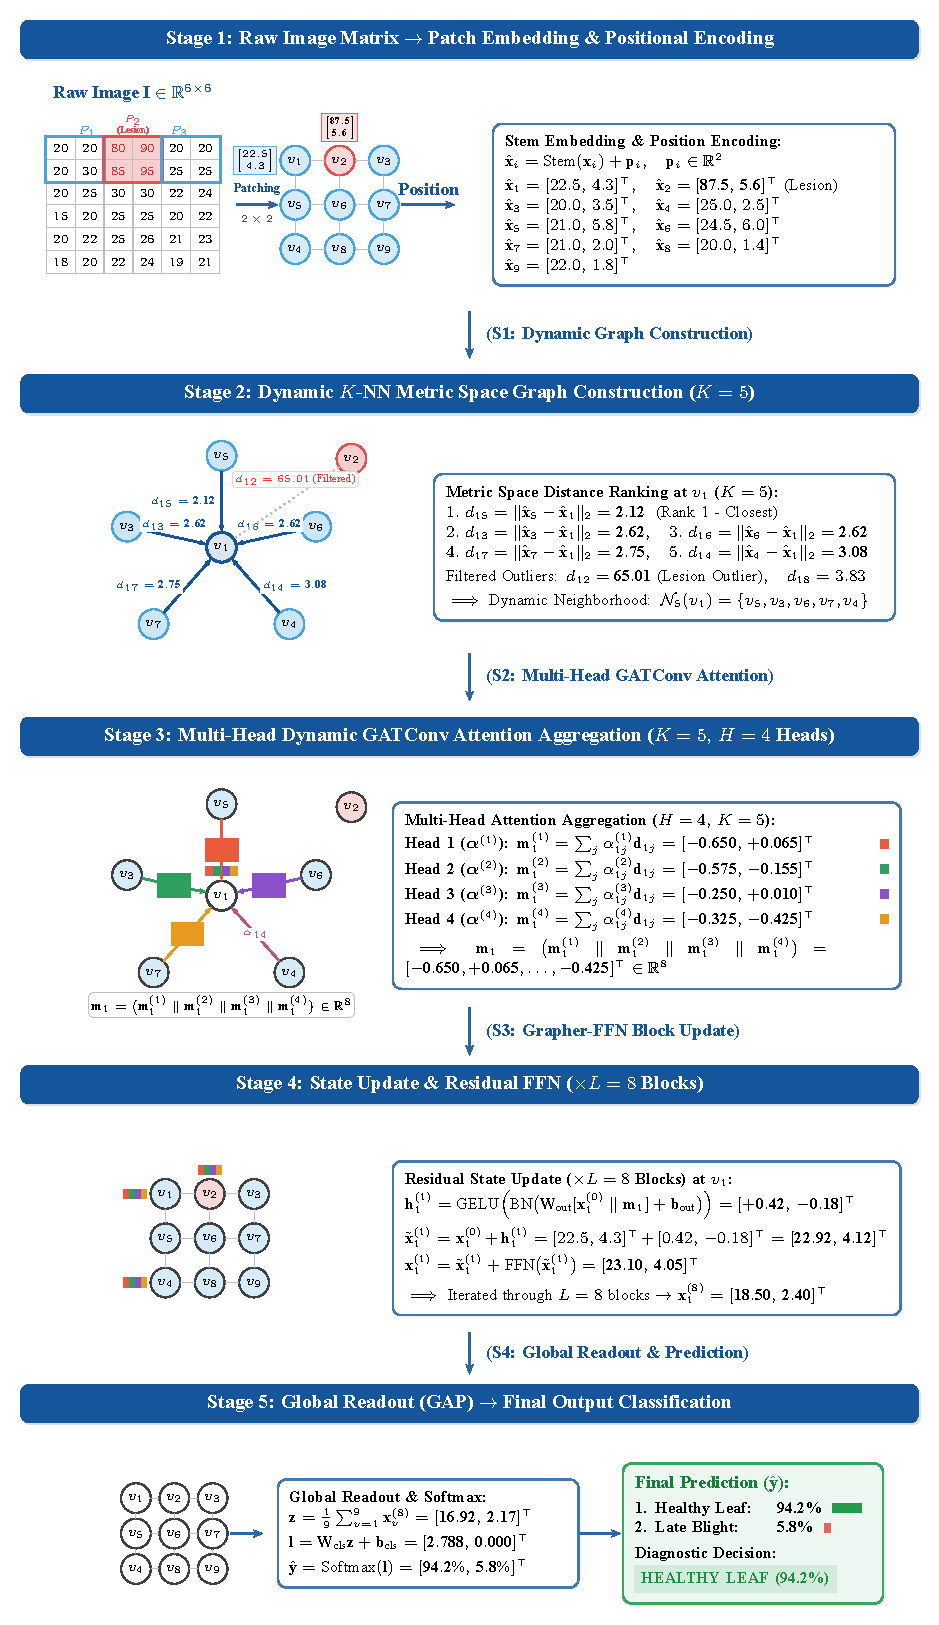
\includegraphics[width=1\textwidth, height=0.95\textheight, keepaspectratio]{figures/Figure_04_concrete_example_flowchart.pdf}
\caption{Step-by-step numerical calculation flowchart of ViGATs across five stages ($K=5$ neighbors, $H=4$ attention heads, and $L=8$ Grapher blocks): from raw pixel matrix and spatial patching, through dynamic metric space graph construction, multi-head edge-difference attention aggregation, residual state updating, to global average pooling and final disease classification.}
\label{fig:dataflow_pipeline}
\end{figure}

\begin{table}[H]
\centering
\small
\tbl{Default hyperparameter configuration of ViGATs.}
{\begin{tabular}{llll} \toprule
\textbf{Symbol} & \textbf{Description} & \textbf{Value} & \textbf{Code reference} \\ \midrule
$C$ & Hidden channels & 192 & \texttt{ch=192} \\
$K$ & KNN neighbors & 5 & \texttt{k=5} \\
$L$ & Grapher--FFN blocks & 8 & \texttt{nb=8} \\
$H$ & Attention heads & 4 & \texttt{heads=4} \\
$d_k$ & Key dim per head & 24 & \texttt{head\_dim=24} \\
$D$ & Attention hidden dim & 96 & $H \cdot d_k$ \\
$N$ & Nodes ($64\times64$ input) & 256 & $(H_0/4)^2$ \\
FFN exp. & FFN expansion ratio & 4 & \texttt{exp=4} \\
Out groups & Output proj. groups & 4 & \texttt{groups=4} \\
$\sigma$ & Attn. activation & LeakyReLU(0.2) & \texttt{nn.LeakyReLU(0.2)} \\
\bottomrule
\end{tabular}}
\label{tab:vigats_config}
\end{table}

\section{Experimental Setup}
\label{sec:experimental-setup}

\subsection{Datasets and Acquisition Conditions}

The experimental design encompasses complementary environmental conditions (summarized in Table~\ref{tab:datasets}): laboratory-controlled imagery (PlantVillage \citep{hughes2015plantvillage}, Rice Leaf Disease V2 \citep{rice_dataset2022}), real-world in-field imagery (Maize Leaf Disease \citep{mduma2023maize}), and an unseen cross-domain target set (IIITDMJ Maize \citep{iiitdmj2024dataset}). Tiny ImageNet \citep{le2015tiny} serves as a general-purpose vision benchmark. All images are standardized to $64 \times 64$ resolution.

\begin{table}[H]
\centering
\small
\tbl{Summary of the datasets used in the experiments.}
{\begin{tabular}{lcccc} \toprule
\textbf{Dataset} & \textbf{Classes} & \textbf{Images} & \textbf{Domain / Type} & \textbf{Resolution} \\ \midrule
PlantVillage \citep{hughes2015plantvillage} & 38 & 54,305 & Lab-controlled & $64 \times 64$ \\
Maize Leaf Disease \citep{mduma2023maize} & 4 & 15,350 & In-field & $64 \times 64$ \\
Rice Leaf Disease V2 \citep{rice_dataset2022} & 4 & 5,932 & Lab-controlled & $64 \times 64$ \\
PlantRaw \citep{tongle2026plantraw} & 35 & 16,165 & In-field multi-crop & $64 \times 64$ \\
Tiny ImageNet \citep{le2015tiny} & 200 & 110,000 & General vision & $64 \times 64$ \\ \midrule
\textbf{IIITDMJ Maize} \citep{iiitdmj2024dataset} & \textbf{4} & \textbf{1,432} & \textbf{Cross-domain benchmark} & \textbf{$64 \times 64$} \\
\quad $\llcorner$ Close-up Leaf (Source domain) & 4 & 416 & In-field close-up leaf & $64 \times 64$ \\
\quad $\llcorner$ Augmented Leaf (CycleGAN) & 4 & 816 & Synthetic augmented leaf & $64 \times 64$ \\
\quad $\llcorner$ Drone Aerial (Target domain) & 4 & 200 & Unseen aerial drone & $64 \times 64$ \\ \bottomrule
\end{tabular}}
\label{tab:datasets}
\end{table}

\subsubsection{PlantRaw: In-the-Wild Multicrop Benchmark}
PlantRaw represents a primary dataset contribution of this work, compiled and standardized across 9 open sources \citep{tongle2026plantraw}. It comprises 16,165 images across 35 disease classes from 10 distinct crops (Table~\ref{tab:plantraw_sources}).

\begin{table}[H]
\footnotesize
\setlength{\tabcolsep}{4pt}
\renewcommand{\arraystretch}{1.08}
\tbl{Composition and sources of the PlantRaw benchmark dataset.}
{\begin{tabular}{@{}p{5.8cm}p{3.0cm}rr@{}} \toprule
\textbf{Data Source} & \textbf{Crop} & \textbf{Classes} & \textbf{Images} \\ \midrule
PlantVillage \citep{hughes2015plantvillage} & Apple, Maize & 8 & 7,023 \\
iCassava \citep{mwebaze2019icassava} & Cassava & 5 & 4,000 \\
Ethiopian Coffee Leaf Disease \citep{yoseph2023coffee} & Coffee & 4 & 1,200 \\
Soybean Diseased Leaf \citep{mishra2023soybean} & Soybean & 4 & 445 \\
Sugarcane Leaf Disease \citep{daphal2022sugarcane} & Sugarcane & 5 & 2,521 \\
Wheat Leaf Dataset \citep{getch2021wheat} & Wheat & 3 & 407 \\
Cucumber Plant Diseases \citep{negm2021cucumber} & Cucumber & 2 & 469 \\
Chili Plant Disease \citep{prakoso2021chili} & Chili & 2 & 20 \\
Rice Leaf Diseases \citep{prajapati2017rice} & Rice & 2 & 80 \\ \midrule
\textbf{Total} & \textbf{10 crops} & \textbf{35} & \textbf{16,165} \\ \bottomrule
\end{tabular}}
\label{tab:plantraw_sources}
\end{table}

Figure~\ref{fig:plantraw_composition} illustrates the distribution of images and classes across crops in PlantRaw.

\begin{figure}[H]
\centering
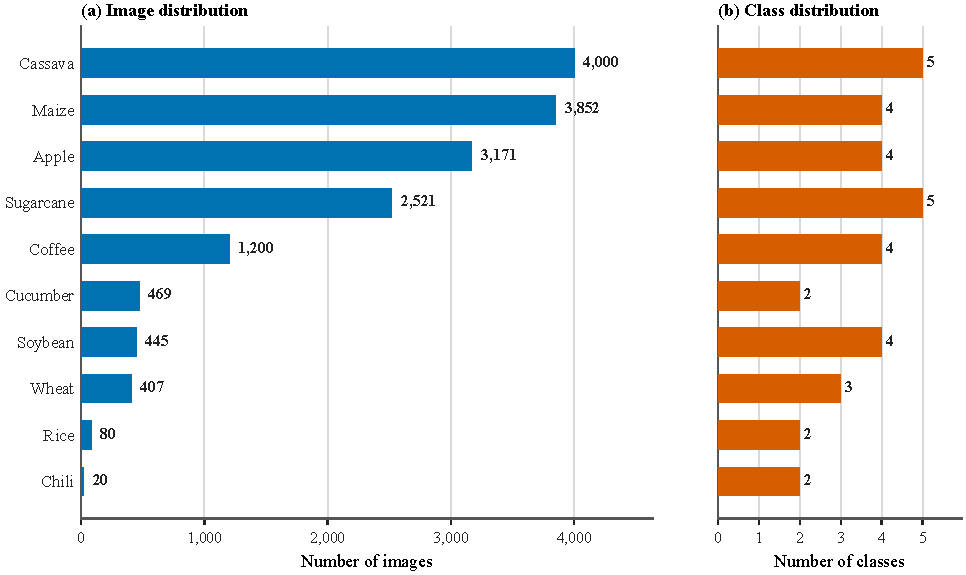
\includegraphics[width=\textwidth]{figures/Figure_05_plantraw_composition.pdf}
\caption{Distribution of images and classes in PlantRaw. Colored bars indicate image counts, and hatched bars indicate the corresponding number of classes.}
\label{fig:plantraw_composition}
\end{figure}

\subsection{Training Protocol and Experimental Rigor}
\label{subsec:training-protocol}

To ensure complete fairness and eliminate data leakage, all architectures are trained from scratch under identical hyperparameter configurations detailed in Table~\ref{tab:training_protocol}. A strict Stratified 5-Fold Cross-Validation protocol is applied across the five core benchmarks (70\% train, 10\% validation, 20\% test). Model checkpoints are selected strictly based on validation performance before evaluating on held-out test splits.

\begin{table}[H]
\footnotesize
\setlength{\tabcolsep}{3.5pt}
\renewcommand{\arraystretch}{1.10}
\tbl{Summary of training protocol, data preprocessing, and experimental setup (Part 1).}
{\begin{tabular}{@{}p{3.1cm}p{5.4cm}p{5.7cm}@{}} \toprule
\textbf{Component} & \textbf{Common Configuration} & \textbf{Dataset-Specific Tuning} \\ \midrule
\multicolumn{3}{l}{\textit{A. Training Protocol and Optimization}} \\ \midrule
Loss function & Cross-Entropy Loss & Label smoothing $\epsilon = 0.1$ on Maize, Rice V2, PlantRaw, Tiny ImageNet, IIITDMJ; none on PlantVillage. \\
Optimizer & AdamW ($\beta_1 = 0.9, \beta_2 = 0.999, \epsilon = 10^{-8}$) & Weight decay $= 0.05$ on PlantVillage; $10^{-4}$ on remaining datasets. \\
Learning rate (LR) & Initial $\eta_0 = 10^{-3}$, no warm-up & Cosine Annealing ($T_{\max} = 100$), decaying to $\eta_{\min} = 10^{-6}$. \\
Batch size & Auto-optimized by VRAM ($\{256, 128, 64, 32, 16\}$) & Batch size 256 on 5 main benchmarks; batch size 64 on IIITDMJ and Ablation. \\
Epochs \& Early stopping & Max 100 epochs; Early stopping on $\text{val\_acc}$ & Patience $= 15$ epochs (Patience $= 20$ on IIITDMJ). \\
Precision & AMP enabled for PlantVillage benchmark and ablation experiments & Standard FP32 precision for remaining benchmarks. \\ \bottomrule
\end{tabular}}
\end{table}

\begin{table}[H]
\addtocounter{table}{-1}
\footnotesize
\setlength{\tabcolsep}{3.5pt}
\renewcommand{\arraystretch}{1.10}
\tbl{Summary of training protocol, data preprocessing, and experimental setup (Part 2).}
{\begin{tabular}{@{}p{3.1cm}p{5.4cm}p{5.7cm}@{}} \toprule
\textbf{Component} & \textbf{Common Configuration} & \textbf{Dataset-Specific Tuning} \\ \midrule
\multicolumn{3}{l}{\textit{B. Data Preprocessing and Partitioning}} \\ \midrule
Input resolution & $64 \times 64 \times 3$ RGB & Fixed resize, ImageNet normalization ($\mu, \sigma$). \\
Data augmentation & Horizontal/vertical flip ($p=0.5$), rotation $\pm 15^\circ$, Color Jitter & RandomAffine (5\%) on PlantVillage; rotation $\pm 30^\circ$ and Grayscale on IIITDMJ. \\
Data split & Main benchmarks: Stratified 5-Fold CV ($\text{seed}=42$), approx. 70\% Train / 10\% Val / 20\% Test & Ablation $K$: 80\% Train / 20\% Val on fixed split; IIITDMJ: source 80\%/20\% per fold, drone target held out. \\
Weight initialization & Training from scratch & Kaiming Normal (Conv/Linear); Truncated Normal (ViT Pos/Cls). \\ \midrule
\multicolumn{3}{l}{\textit{C. Implementation Environment}} \\ \midrule
Hardware platform & \multicolumn{2}{p{11.1cm}}{Intel Core i5-13400F CPU, 32 GB DDR5 RAM, NVIDIA GeForce RTX 5070 Ti GPU (16 GB VRAM), 500 GB NVMe SSD.} \\
Operating system & \multicolumn{2}{p{11.1cm}}{Ubuntu 24.04 LTS, 64-bit.} \\
Software stack & \multicolumn{2}{p{11.1cm}}{Python 3.12.10, PyTorch with CUDA acceleration, torchvision, Pillow, NumPy, pandas, scikit-learn, thop 0.1.1.} \\ \bottomrule
\end{tabular}}
\label{tab:training_protocol}
\parbox{\textwidth}{\vspace{2pt}\footnotesize\textit{Note:} AMP: Automatic Mixed Precision; LR: Learning Rate; VRAM: Video Random Access Memory; CV: Cross-Validation. Main benchmarks use \texttt{num\_workers}=4; IIITDMJ uses \texttt{num\_workers}=0. \texttt{pin\_memory=True} is enabled during data loading.}
\end{table}

\subsection{Benchmark Baselines}
The benchmark baseline models representing four major architecture families (CNN, ViT, SSM, GNN) and three modern lightweight architectures are detailed in Table~\ref{tab:benchmark_models}.

\begin{table}[H]
\small
\setlength{\tabcolsep}{3.0pt}
\renewcommand{\arraystretch}{1.15}
\tbl{Benchmark models, roles in experimental design, and evaluation scope. ``Four plant datasets'' denotes PlantVillage, Maize Disease, Rice Leaf V2, and PlantRaw.}
{\begin{tabular}{@{}p{1.55cm}p{4.70cm}p{5.55cm}p{2.65cm}@{}} \toprule
\textbf{Family} & \textbf{Model} & \textbf{Benchmark Role} & \textbf{Evaluation Scope} \\ \midrule
\multirow{3}{*}{CNN}
 & ResNet-18 \citep{he2016deep} & Standard residual CNN baseline. & Four plant datasets + Tiny ImageNet \\
 & ConvNeXt-Tiny \citep{liu2022convnext} & Modernized CNN with next-gen conv design. & Four plant datasets + Tiny ImageNet \\
 & EfficientNetV2-S \citep{tan2021efficientnetv2} & Efficiency-optimized CNN baseline. & Four plant datasets + Tiny ImageNet \\ \midrule
\multirow{2}{*}{Transformer}
 & ViT \citep{dosovitskiy2020image} & Standard ViT with global self-attention. & Four plant datasets + Tiny ImageNet \\
 & Swin-T \citep{liu2021swin} & Hierarchical shifted-window Transformer. & Four plant datasets + Tiny ImageNet \\ \midrule
SSM
 & MambaOut-Tiny \citep{yu2024mambaout} & Gated conv model testing vision SSMs. & Four plant datasets + Tiny ImageNet \\ \midrule
\multirow{3}{*}{GNN}
 & ViG \citep{han2022vision} & Vision GNN with MRConv (base of ViGATs). & Four plant datasets + Tiny ImageNet \\
 & ViG+GAT \citep{velickovic2018graph} & Variant replacing MRConv with standard GAT. & Four plant datasets + Tiny ImageNet \\
 & ViG+GATv2 \citep{brody2022gat} & Variant with dynamic GATv2 attention. & Four plant datasets + Tiny ImageNet \\ \midrule
\multirow{3}{*}{Lightweight}
 & FastViT-T8 \citep{vasu2023fastvit} & Structural re-parameterization hybrid. & Tiny ImageNet \\
 & RepViT-M1 \citep{wang2024repvit} & Mobile CNN from a ViT perspective. & Tiny ImageNet \\
 & EfficientViT-B1 \citep{cai2023efficientvit} & Multi-scale efficient attention model. & Tiny ImageNet \\ \bottomrule
\end{tabular}}
\label{tab:benchmark_models}
\end{table}

\subsection{Evaluation Metrics and Statistical Testing}
\label{subsec:evaluation_metrics}

Performance is quantified via standard confusion matrix metrics \citep{sokolova2009systematic}. All 5-fold cross-validation metrics are reported as sample mean and standard deviation ($\bar{M} \pm s$):
\begin{equation}
\bar{M} = \frac{1}{K_{\mathrm{fold}}} \sum_{k=1}^{K_{\mathrm{fold}}} M_k, \qquad
s = \sqrt{\frac{1}{K_{\mathrm{fold}} - 1} \sum_{k=1}^{K_{\mathrm{fold}}} (M_k - \bar{M})^2}.
\end{equation}
Statistical significance between ViGATs and baseline models is verified using Holm-adjusted paired $t$-tests ($p_{\mathrm{Holm}}$).


\section{Experimental Results and Analysis}
\label{sec:results}

\subsection{Ablation Studies}
\label{sec:ablation}

We investigate the sensitivity of ViGATs to key architectural hyper-parameters on PlantVillage. Table~\ref{tab:ablation_k} demonstrates that $K=5$ neighbors achieves optimal performance ($99.82\%$ accuracy) while maintaining low latency ($0.98$ ms).

\begin{table}[H]
\small
\tbl{Validation performance across different numbers of graph neighbors $K$ on PlantVillage.}
{\begin{tabular}{lccccc} \toprule
\textbf{Model} & \textbf{$K=3$} & \textbf{$K=5$ (Default)} & \textbf{$K=7$} & \textbf{$K=9$} & \textbf{Latency (ms)} \\ \midrule
ViG \citep{han2022vision} & \secondresult{99.77\%} & \secondresult{99.77\%} & \bestresult{99.82\%} & \bestresult{99.80\%} & \bestresult{0.92} \\
ViGATs (Proposed) & \bestresult{99.78\%} & \bestresult{99.82\%} & \secondresult{99.76\%} & \bestresult{99.80\%} & \secondresult{0.98} \\ \bottomrule
\end{tabular}}
\label{tab:ablation_k}
\parbox{\textwidth}{\vspace{2pt}\footnotesize\textit{Note:} \bestresult{Green bold} and \secondresult{orange} values denote the best and second-best result in each column; tied best values are both shown in green. Lower latency is better.}
\end{table}

Table~\ref{tab:ablation_ext} presents an extended one-factor-at-a-time ablation on attention heads $H$, depth $L$, channels $C$, and attention activations $\sigma$.

\begin{table}[H]
\footnotesize
\setlength{\tabcolsep}{4pt}
\tbl{Extended one-factor-at-a-time ablation of GATConv on a fixed PlantVillage split. The final ViGATs configuration selected for subsequent experiments is marked by $\dagger$.}
{\begin{tabular}{llccccc} \toprule
\textbf{Factor} & \textbf{Configuration} & \textbf{AC (\%)} & \textbf{F1 (\%)} & \textbf{Params (M)} & \textbf{Epochs} & \textbf{Time/Epoch (s)} \\ \midrule
\multirow{4}{*}{Attention heads ($H$)} & $H=1$ & 99.65 & 99.51 & 4.67 & 90 & 37.1 \\
 & $H=2$ & \secondresult{99.67} & \secondresult{99.61} & 4.67 & 95 & 36.6 \\
 & $H=4^{\dagger}$ & \bestresult{99.72} & \bestresult{99.64} & 4.67 & 98 & 36.6 \\
 & $H=8$ & 99.48 & 99.38 & 4.67 & 84 & 36.0 \\
\midrule
\multirow{4}{*}{Grapher--FFN blocks ($L$)} & $L=4$ & \secondresult{99.70} & \secondresult{99.59} & 2.73 & 96 & 19.7 \\
 & $L=6$ & 98.44 & 97.48 & 3.70 & 37 & 27.8 \\
 & $L=8^{\dagger}$ & \bestresult{99.72} & \bestresult{99.64} & 4.67 & 98 & 36.6 \\
 & $L=12$ & 99.25 & 98.95 & 6.61 & 60 & 53.7 \\
\midrule
\multirow{4}{*}{Hidden dimension ($C$)} & $C=96$ & 99.71 & 99.54 & 1.27 & 100 & 3.6 \\
 & $C=144$ & \secondresult{99.74} & \bestresult{99.68} & 2.70 & 100 & 30.0 \\
 & $C=192^{\dagger}$ & 99.72 & 99.64 & 4.67 & 98 & 36.6 \\
 & $C=256$ & \bestresult{99.76} & \secondresult{99.67} & 8.14 & 100 & 47.3 \\
\midrule
\multirow{3}{*}{Activation} & LeakyReLU$^{\dagger}$ & \bestresult{99.72} & \bestresult{99.64} & 4.67 & 98 & 36.6 \\
 & GELU & 99.66 & 99.52 & 4.67 & 100 & 39.8 \\
 & ReLU & \secondresult{99.71} & \secondresult{99.58} & 4.67 & 100 & 36.1 \\
\bottomrule
\end{tabular}}
\label{tab:ablation_ext}
\parbox{\textwidth}{\vspace{2pt}\footnotesize\textit{Note:} Within each factor group, \bestresult{green bold} and \secondresult{orange} values denote the best and second-best AC/F1 result. The $\dagger$ setting defines the final ViGATs configuration used in the benchmark experiments. Time/Epoch is the recorded training time divided by the number of completed epochs under the identical hardware environment.}
\end{table}

\subsection{Plant Disease Benchmarks}
\label{sec:plant_disease_benchmarks}

Table~\ref{tab:three_benchmark_datasets} reports 5-fold cross-validation performance across PlantVillage, Maize Disease, and Rice Leaf V2.

\begin{table}[H]
\footnotesize
\setlength{\tabcolsep}{3.0pt}
\tbl{Classification performance (mean $\pm$ sample standard deviation, \%) on three plant-disease datasets using 5-Fold CV.}
{\begin{tabular}{lccccc} \toprule
\textbf{Approach} & \textbf{AC (\%)} & \textbf{PR (\%)} & \textbf{RE (\%)} & \textbf{F1 (\%)} & \textbf{$p_{\mathrm{Holm}}$} \\ \midrule
\multicolumn{6}{c}{\textbf{(a) PlantVillage (38 classes, 54,305 images)}} \\ \midrule
ResNet-18 \citep{he2016deep} & $99.39 \pm 0.12$ & $99.17 \pm 0.14$ & $99.09 \pm 0.18$ & $99.13 \pm 0.14$ & 0.007 \\
ConvNeXt-Tiny \citep{liu2022convnext} & $97.99 \pm 0.23$ & $97.28 \pm 0.39$ & $97.09 \pm 0.32$ & $97.17 \pm 0.34$ & 0.001 \\
EfficientNetV2-S \citep{tan2021efficientnetv2} & $99.39 \pm 0.12$ & $99.14 \pm 0.23$ & $99.05 \pm 0.25$ & $99.09 \pm 0.24$ & 0.041 \\
ViT \citep{dosovitskiy2020image} & $99.31 \pm 0.12$ & $99.08 \pm 0.15$ & $98.96 \pm 0.21$ & $99.01 \pm 0.18$ & 0.007 \\
Swin-T \citep{liu2021swin} & $98.83 \pm 0.19$ & $98.39 \pm 0.26$ & $98.24 \pm 0.24$ & $98.30 \pm 0.23$ & 0.006 \\
MambaOut-Tiny \citep{yu2024mambaout} & $81.28 \pm 39.77$ & $79.01 \pm 44.02$ & $79.41 \pm 42.92$ & $79.01 \pm 43.90$ & 0.701 \\
ViG \citep{han2022vision} & \secondresult{$99.68 \pm 0.07$} & \secondresult{$99.58 \pm 0.11$} & \secondresult{$99.55 \pm 0.13$} & \secondresult{$99.56 \pm 0.10$} & 0.701 \\
ViG+GAT \citep{velickovic2018graph} & $99.60 \pm 0.18$ & $99.48 \pm 0.22$ & $99.41 \pm 0.30$ & $99.44 \pm 0.25$ & 0.273 \\
ViG+GATv2 \citep{brody2022gat} & $99.55 \pm 0.38$ & $99.34 \pm 0.51$ & $99.35 \pm 0.51$ & $99.34 \pm 0.51$ & 0.701 \\
ViGATs (Proposed) & \bestresult{$99.75 \pm 0.06$} & \bestresult{$99.66 \pm 0.09$} & \bestresult{$99.63 \pm 0.09$} & \bestresult{$99.64 \pm 0.07$} & --- (Ref.) \\
\midrule
\multicolumn{6}{c}{\textbf{(b) Maize Leaf Disease (4 classes, 15,350 images)}} \\ \midrule
ResNet-18 \citep{he2016deep} & $97.27 \pm 0.34$ & $96.73 \pm 0.39$ & $96.98 \pm 0.47$ & $96.85 \pm 0.40$ & $< 0.001$ \\
ConvNeXt-Tiny \citep{liu2022convnext} & $95.77 \pm 0.49$ & $94.98 \pm 0.66$ & $95.15 \pm 0.54$ & $95.05 \pm 0.59$ & $< 0.001$ \\
EfficientNetV2-S \citep{tan2021efficientnetv2} & $95.64 \pm 0.38$ & $94.80 \pm 0.50$ & $94.88 \pm 0.55$ & $94.83 \pm 0.48$ & $< 0.001$ \\
ViT \citep{dosovitskiy2020image} & $93.97 \pm 0.59$ & $93.01 \pm 0.60$ & $92.93 \pm 0.80$ & $92.97 \pm 0.69$ & $< 0.001$ \\
Swin-T \citep{liu2021swin} & $71.03 \pm 23.70$ & $60.15 \pm 35.82$ & $64.01 \pm 31.47$ & $59.23 \pm 36.80$ & 0.183 \\
MambaOut-Tiny \citep{yu2024mambaout} & $59.97 \pm 21.04$ & $32.93 \pm 35.94$ & $46.13 \pm 28.61$ & $37.36 \pm 33.48$ & 0.057 \\
ViG \citep{han2022vision} & $98.11 \pm 0.37$ & $97.84 \pm 0.47$ & $97.89 \pm 0.57$ & $97.85 \pm 0.44$ & 0.005 \\
ViG+GAT \citep{velickovic2018graph} & $98.34 \pm 0.11$ & $98.04 \pm 0.15$ & $98.19 \pm 0.19$ & $98.11 \pm 0.13$ & 0.294 \\
ViG+GATv2 \citep{brody2022gat} & \secondresult{$98.55 \pm 0.47$} & \bestresult{$98.34 \pm 0.51$} & \secondresult{$98.36 \pm 0.57$} & \secondresult{$98.35 \pm 0.54$} & 0.841 \\
ViGATs (Proposed) & \bestresult{$98.58 \pm 0.39$} & \secondresult{$98.32 \pm 0.48$} & \bestresult{$98.44 \pm 0.42$} & \bestresult{$98.38 \pm 0.45$} & --- (Ref.) \\
\midrule
\multicolumn{6}{c}{\textbf{(c) Rice Leaf Disease V2 (4 classes, 5,932 images)}} \\ \midrule
ResNet-18 \citep{he2016deep} & $99.88 \pm 0.11$ & $99.88 \pm 0.12$ & $99.89 \pm 0.11$ & $99.88 \pm 0.11$ & 1.000 \\
ConvNeXt-Tiny \citep{liu2022convnext} & $99.81 \pm 0.28$ & $99.82 \pm 0.28$ & $99.82 \pm 0.27$ & $99.82 \pm 0.28$ & 1.000 \\
EfficientNetV2-S \citep{tan2021efficientnetv2} & $99.70 \pm 0.16$ & $99.70 \pm 0.16$ & $99.70 \pm 0.17$ & $99.70 \pm 0.16$ & 0.561 \\
ViT \citep{dosovitskiy2020image} & $99.29 \pm 0.77$ & $99.32 \pm 0.75$ & $99.30 \pm 0.77$ & $99.31 \pm 0.77$ & 0.711 \\
Swin-T \citep{liu2021swin} & $39.09 \pm 3.87$ & $29.38 \pm 6.53$ & $37.86 \pm 4.22$ & $29.26 \pm 4.50$ & $< 0.001$ \\
MambaOut-Tiny \citep{yu2024mambaout} & $56.15 \pm 39.95$ & $44.01 \pm 51.03$ & $54.97 \pm 41.03$ & $46.34 \pm 48.91$ & 0.561 \\
ViG \citep{han2022vision} & $99.88 \pm 0.18$ & $99.89 \pm 0.18$ & $99.88 \pm 0.19$ & $99.88 \pm 0.19$ & 1.000 \\
ViG+GAT \citep{velickovic2018graph} & $99.76 \pm 0.26$ & $99.78 \pm 0.23$ & $99.76 \pm 0.27$ & $99.77 \pm 0.25$ & 0.561 \\
ViG+GATv2 \citep{brody2022gat} & \secondresult{$99.92 \pm 0.12$} & \secondresult{$99.92 \pm 0.12$} & \secondresult{$99.92 \pm 0.12$} & \secondresult{$99.92 \pm 0.12$} & 1.000 \\
ViGATs (Proposed) & \bestresult{$99.93 \pm 0.11$} & \bestresult{$99.93 \pm 0.11$} & \bestresult{$99.93 \pm 0.11$} & \bestresult{$99.93 \pm 0.11$} & --- (Ref.) \\
\bottomrule
\end{tabular}}
\label{tab:three_benchmark_datasets}
\parbox{\textwidth}{\vspace{2pt}\footnotesize\textit{Note:} Values are mean $\pm$ sample standard deviation across five folds. \bestresult{Green bold} and \secondresult{orange} values denote the best and second-best result in each metric column. Holm-adjusted paired $t$-tests compare each model with ViGATs.}
\end{table}

\subsubsection{PlantRaw: Multicrop Field Benchmark}
Table~\ref{tab:plantraw} evaluates models on the unconstrained, multicrop PlantRaw dataset. ViGATs maintains the highest accuracy ($86.12\%$), significantly exceeding CNN and Transformer architectures.

\begin{table}[H]
\footnotesize
\setlength{\tabcolsep}{3.0pt}
\tbl{Classification performance (mean $\pm$ sample standard deviation, \%) on PlantRaw (35 classes, 16,165 images) using 5-Fold CV.}
{\begin{tabular}{lccccc} \toprule
\textbf{Approach} & \textbf{AC (\%)} & \textbf{PR (\%)} & \textbf{RE (\%)} & \textbf{F1 (\%)} & \textbf{$p_{\mathrm{Holm}}$} \\ \midrule
ResNet-18 \citep{he2016deep} & $79.64 \pm 0.94$ & $80.77 \pm 3.26$ & $78.93 \pm 2.30$ & $79.25 \pm 2.79$ & $< 0.001$ \\
ConvNeXt-Tiny \citep{liu2022convnext} & $72.97 \pm 1.03$ & $72.00 \pm 0.88$ & $71.33 \pm 1.36$ & $71.30 \pm 1.16$ & $< 0.001$ \\
EfficientNetV2-S \citep{tan2021efficientnetv2} & $75.32 \pm 1.14$ & $74.03 \pm 1.97$ & $73.12 \pm 3.32$ & $73.18 \pm 2.75$ & $< 0.001$ \\
ViT \citep{dosovitskiy2020image} & $70.91 \pm 0.80$ & $71.72 \pm 2.21$ & $70.62 \pm 2.26$ & $70.41 \pm 2.49$ & $< 0.001$ \\
Swin-T \citep{liu2021swin} & $56.63 \pm 13.07$ & $50.37 \pm 16.55$ & $46.70 \pm 17.11$ & $46.00 \pm 18.02$ & 0.041 \\
MambaOut-Tiny \citep{yu2024mambaout} & $63.78 \pm 27.16$ & $59.31 \pm 32.31$ & $59.81 \pm 30.63$ & $58.99 \pm 31.83$ & 0.550 \\
ViG \citep{han2022vision} & $85.01 \pm 2.00$ & $86.52 \pm 4.58$ & $84.89 \pm 4.29$ & $85.19 \pm 4.46$ & 0.572 \\
ViG+GAT \citep{velickovic2018graph} & $85.85 \pm 0.80$ & $87.21 \pm 3.21$ & $86.22 \pm 2.60$ & $86.35 \pm 2.80$ & 0.802 \\
ViG+GATv2 \citep{brody2022gat} & \secondresult{$85.94 \pm 0.79$} & \bestresult{$88.09 \pm 2.21$} & \secondresult{$86.54 \pm 1.70$} & \bestresult{$86.98 \pm 1.81$} & 0.802 \\
ViGATs (Proposed) & \bestresult{$86.12 \pm 0.61$} & \secondresult{$87.76 \pm 3.19$} & \bestresult{$86.72 \pm 2.57$} & \secondresult{$86.87 \pm 2.79$} & --- (Ref.) \\
\bottomrule
\end{tabular}}
\label{tab:plantraw}
\parbox{\textwidth}{\vspace{2pt}\footnotesize\textit{Note:} Values are mean $\pm$ sample standard deviation across five folds. \bestresult{Green bold} and \secondresult{orange} values denote the best and second-best result in each metric column.}
\end{table}

Figure~\ref{fig:plantraw_curves} displays optimization and validation trajectories across models on PlantRaw.

\begin{figure}[H]
\centering
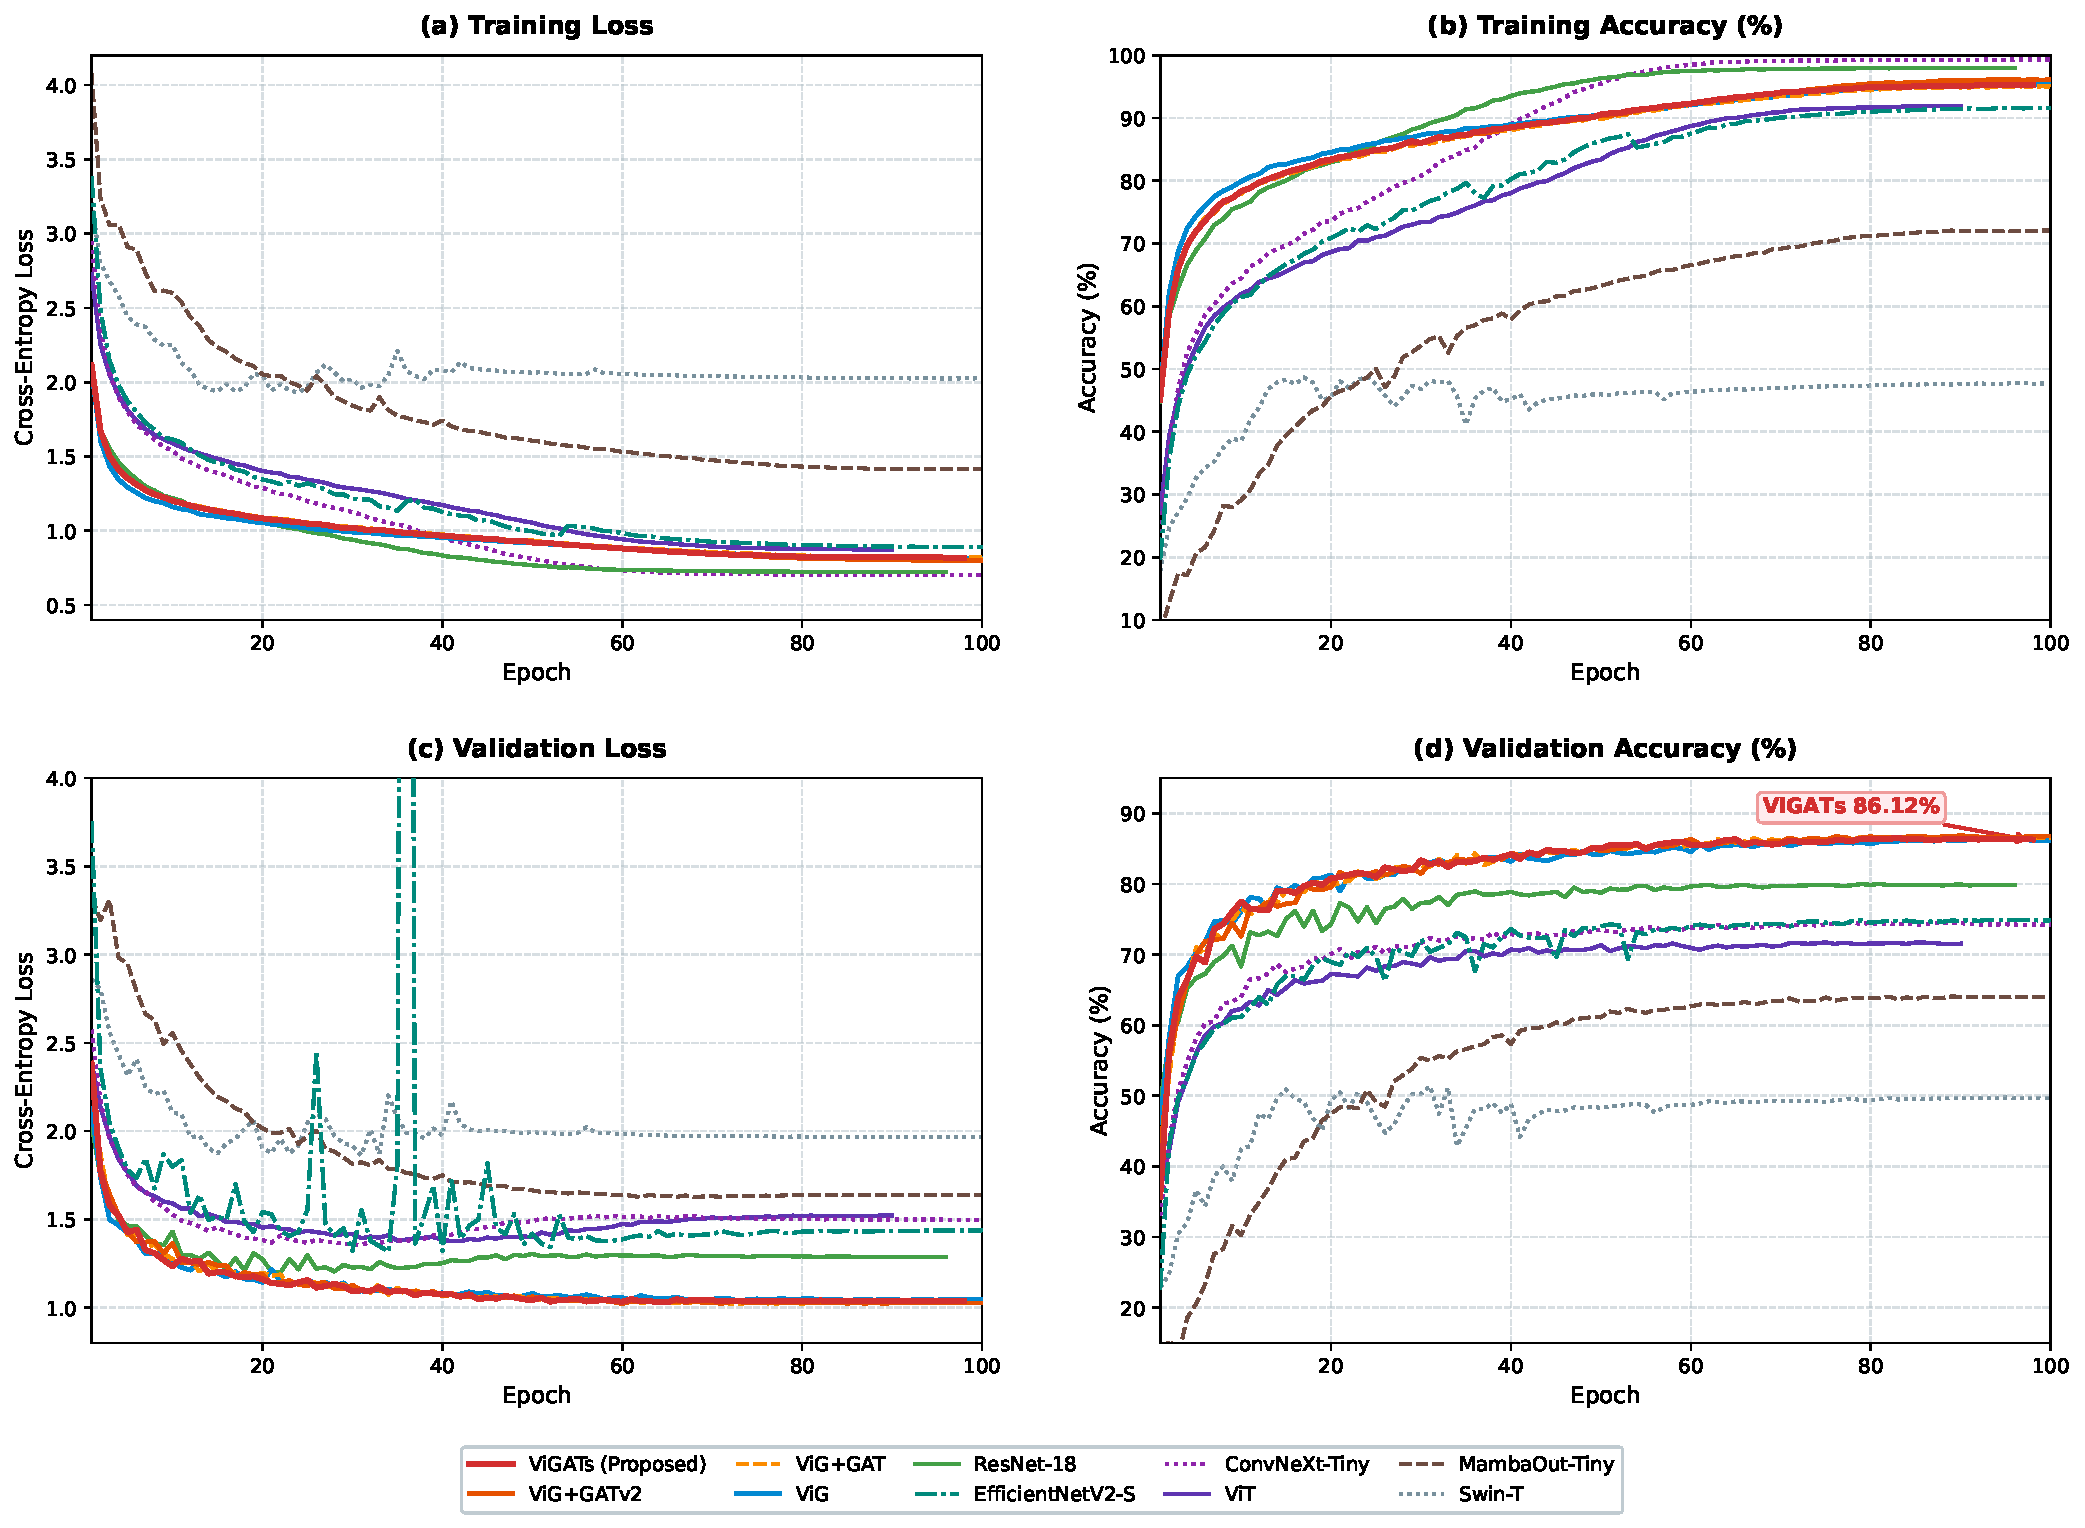
\includegraphics[width=\textwidth]{figures/Figure_06_plantraw_curves.pdf}
\caption{Training and validation curves of the evaluated models on PlantRaw.}
\label{fig:plantraw_curves}
\end{figure}

\subsection{Cross-Domain Transfer to Aerial Drone Imagery}
\label{sec:crossdomain_iiitdmj}

Table~\ref{tab:crossdomain} presents zero-shot transfer performance from close-up field imagery to unseen aerial drone captures on IIITDMJ Maize.

\begin{table}[H]
\footnotesize
\setlength{\tabcolsep}{3.2pt}
\tbl{Cross-domain evaluation on IIITDMJ. Models were trained on close-up images and evaluated without fine-tuning on 200 aerial images (50 images per class).}
{\begin{tabular}{lcccccc} \toprule
\multirow{2}{*}{\textbf{Model}} & \multicolumn{3}{c}{\textbf{Original close-up set}} & \multicolumn{3}{c}{\textbf{Augmented close-up set}} \\ \cmidrule(lr){2-4} \cmidrule(lr){5-7}
 & \textbf{Field (\%)} & \textbf{Drone (\%)} & \textbf{Gap} & \textbf{Field (\%)} & \textbf{Drone (\%)} & \textbf{Gap} \\ \midrule
ResNet-18 \citep{he2016deep} & $90.62 \pm 5.29$ & $66.70 \pm 3.83$ & 23.92 & $96.69 \pm 1.27$ & $67.10 \pm 1.98$ & 29.59 \\
ConvNeXt-Tiny \citep{liu2022convnext} & $85.33 \pm 5.02$ & \bestresult{$77.50 \pm 5.86$} & 7.83 & $93.62 \pm 1.67$ & \bestresult{$77.00 \pm 1.58$} & 16.62 \\
EfficientNetV2-S \citep{tan2021efficientnetv2} & $77.87 \pm 7.09$ & $59.50 \pm 17.91$ & 18.37 & $86.64 \pm 3.35$ & $58.20 \pm 11.86$ & 28.44 \\
ViT \citep{dosovitskiy2020image} & $82.93 \pm 3.59$ & $70.70 \pm 10.40$ & 12.23 & $88.97 \pm 1.16$ & $58.00 \pm 4.34$ & 30.97 \\
Swin-T \citep{liu2021swin} & $57.21 \pm 7.19$ & $55.10 \pm 6.06$ & 2.11 & $51.00 \pm 10.66$ & $55.90 \pm 9.96$ & -4.90 \\
MambaOut-Tiny \citep{yu2024mambaout} & $46.44 \pm 26.30$ & $41.60 \pm 23.60$ & 4.84 & $50.52 \pm 27.98$ & $48.70 \pm 23.54$ & 1.82 \\
ViG \citep{han2022vision} & \bestresult{$93.99 \pm 1.71$} & $63.70 \pm 5.25$ & 30.29 & $96.81 \pm 1.26$ & $64.00 \pm 3.98$ & 32.81 \\
ViG+GAT \citep{velickovic2018graph} & $90.63 \pm 2.59$ & $69.30 \pm 4.60$ & 21.33 & \secondresult{$96.93 \pm 1.89$} & $67.20 \pm 5.44$ & 29.73 \\
ViG+GATv2 \citep{brody2022gat} & \secondresult{$92.30 \pm 1.40$} & $62.80 \pm 4.49$ & 29.50 & $96.57 \pm 1.35$ & $66.60 \pm 7.87$ & 29.97 \\
ViGATs (Proposed) & $90.37 \pm 5.79$ & \secondresult{$71.30 \pm 4.10$} & 19.07 & \bestresult{$97.18 \pm 1.27$} & \secondresult{$69.00 \pm 4.49$} & 28.18 \\
\bottomrule
\end{tabular}}
\label{tab:crossdomain}
\parbox{\textwidth}{\vspace{2pt}\footnotesize\textit{Note:} Values are mean $\pm$ sample standard deviation across five source-domain folds. \bestresult{Green bold} and \secondresult{orange} denote the best and second-best Field/Drone accuracy in each scenario; Gap is unranked. Field denotes close-up test accuracy; Drone denotes accuracy on the fixed 200-image target set; Gap = Field $-$ Drone.}
\end{table}

Figure~\ref{fig:iiitdmj_cm} displays normalized confusion matrices for representative architectures under drone domain shift.

\begin{figure}[H]
\centering
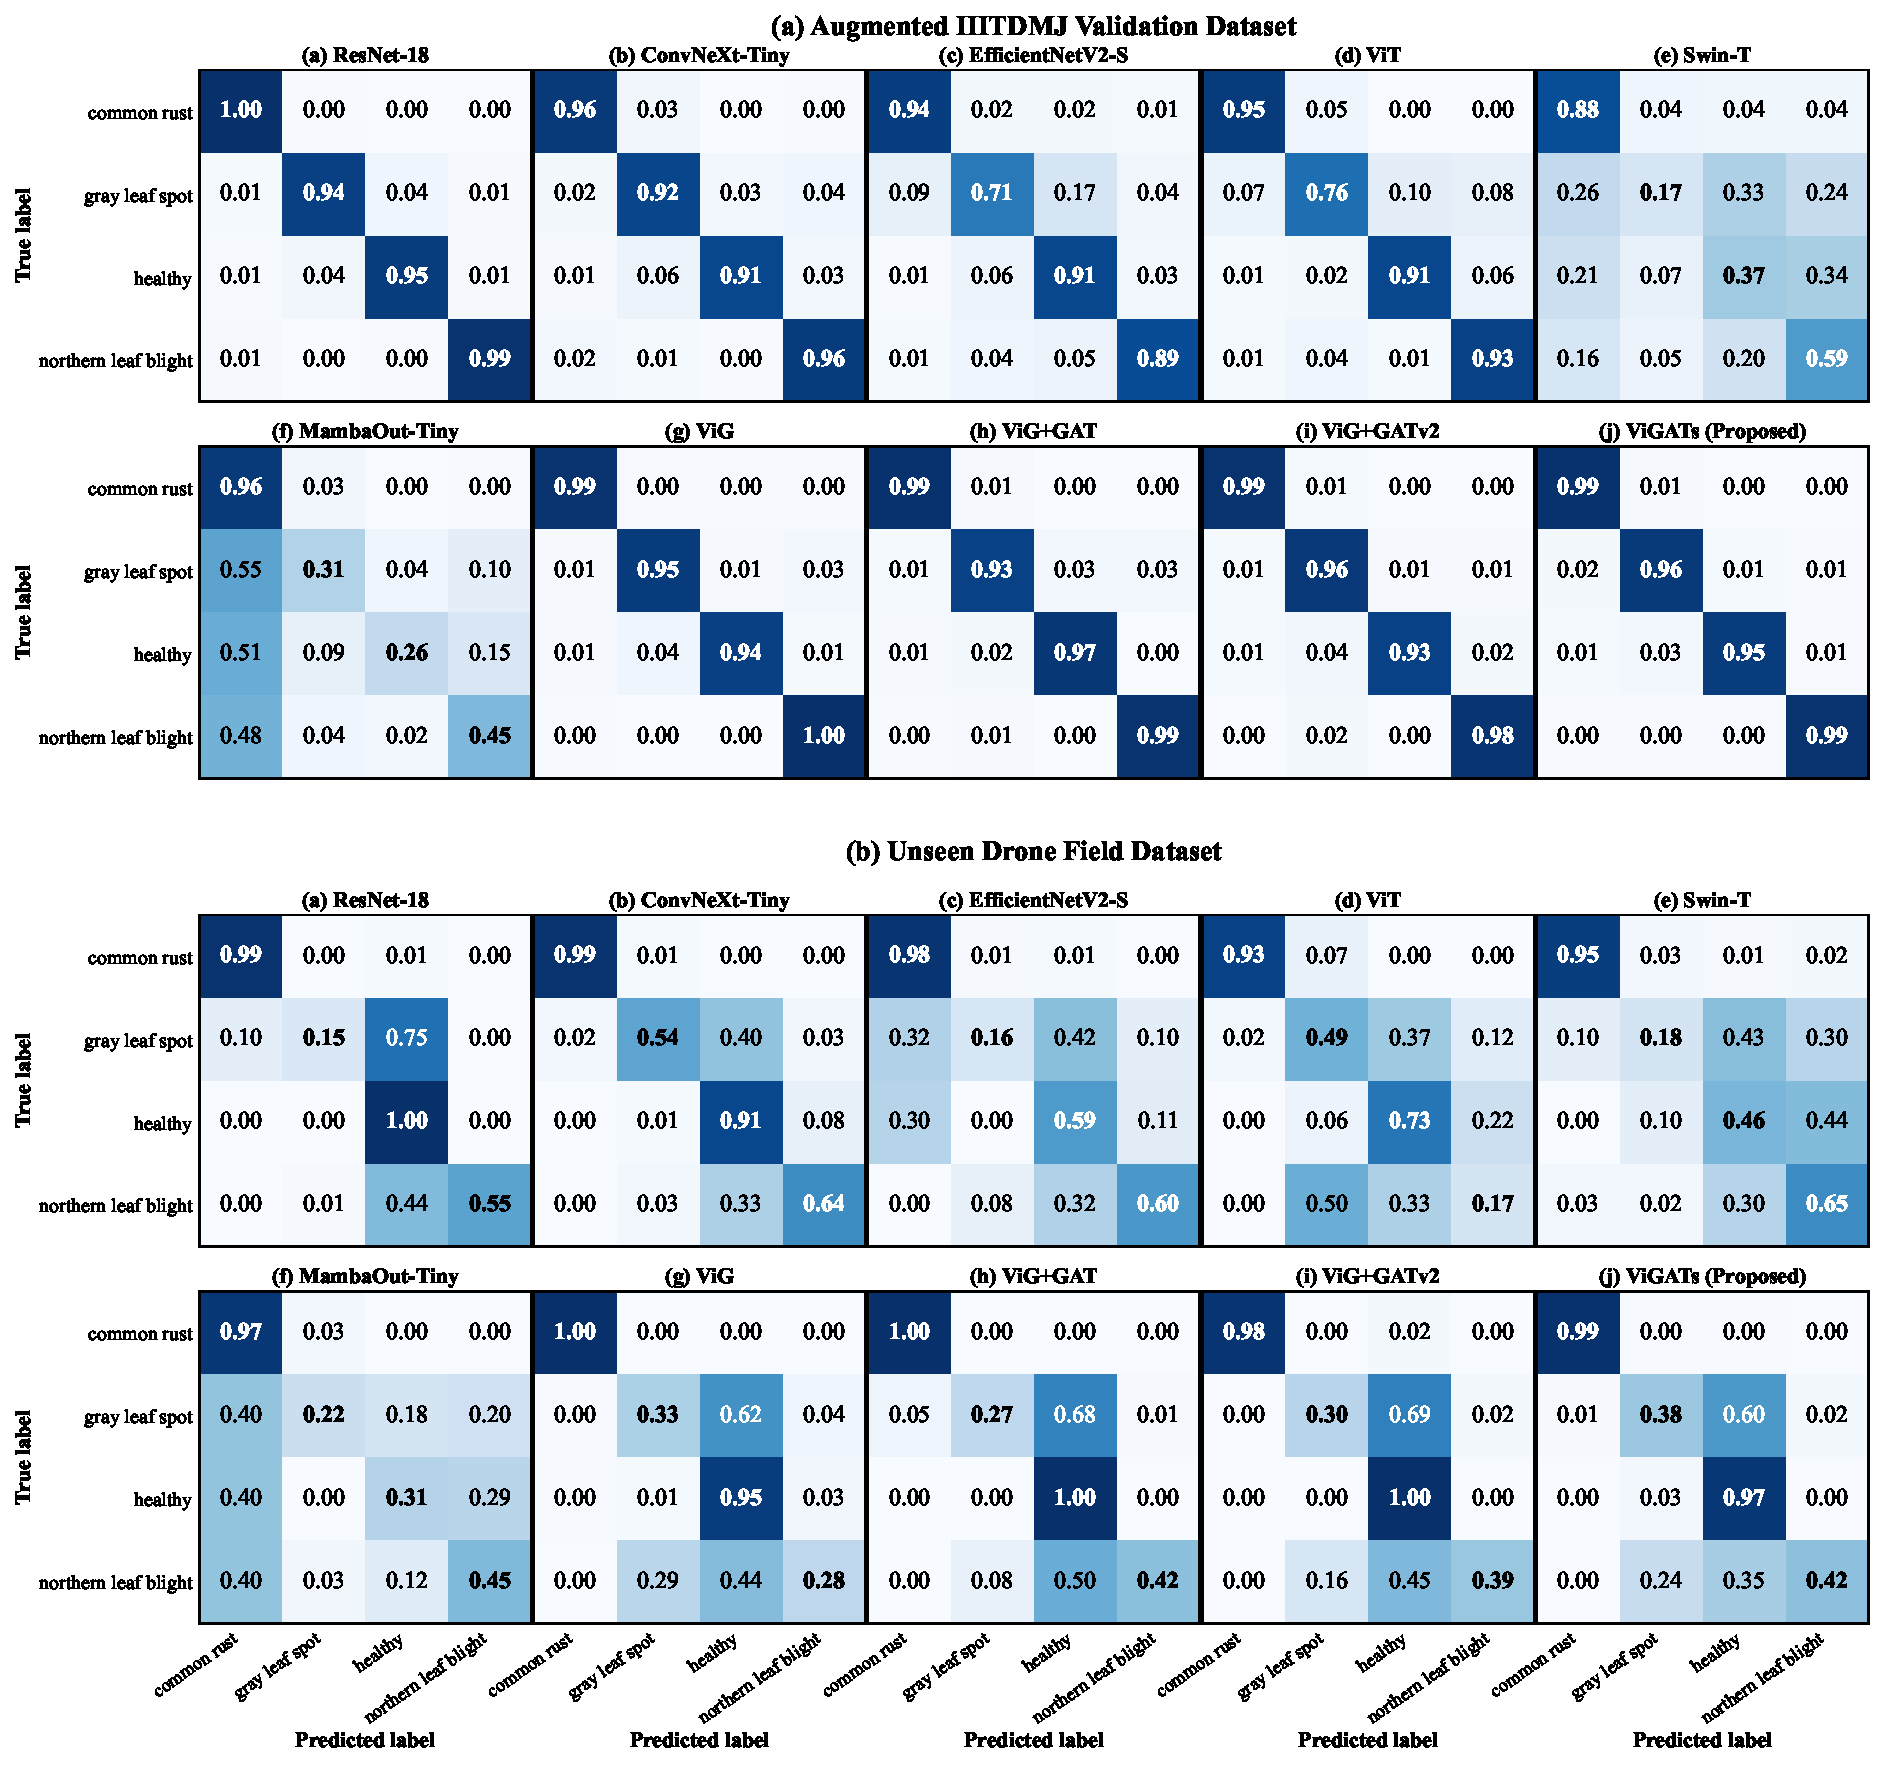
\includegraphics[width=\textwidth]{figures/Figure_07_iiitdmj_confusion_matrices.pdf}
\caption{Confusion Matrices of benchmark models on two evaluation scenarios: (a) the augmented IIITDMJ validation set and (b) the unseen drone field dataset.}
\label{fig:iiitdmj_cm}
\end{figure}

\subsection{General Vision Benchmark: Tiny ImageNet}
\label{sec:tiny_imagenet}

Table~\ref{tab:tiny_imagenet} evaluates the general-purpose visual representation capacity of ViGATs on Tiny ImageNet when trained from scratch at $64 \times 64$ resolution. ViGATs achieves $45.73\%$ accuracy, surpassing the best non-GNN baseline (ResNet-18 at $37.50\%$) and lightweight vision transformers.

\begin{table}[H]
\footnotesize
\setlength{\tabcolsep}{3.0pt}
\tbl{Architectural validation on Tiny ImageNet (200 classes, 110,000 images) using 5-Fold CV and training from scratch at $64 \times 64$ resolution.}
{\begin{tabular}{lccccc} \toprule
\textbf{Approach} & \textbf{AC (\%)} & \textbf{PR (\%)} & \textbf{RE (\%)} & \textbf{F1 (\%)} & \textbf{$p_{\mathrm{Holm}}$} \\ \midrule
ResNet-18 \citep{he2016deep} & \secondresult{$37.50 \pm 1.61$} & \secondresult{$37.72 \pm 0.29$} & \secondresult{$37.50 \pm 1.61$} & \secondresult{$36.88 \pm 1.35$} & 0.001 \\
ConvNeXt-Tiny \citep{liu2022convnext} & $32.51 \pm 0.33$ & $32.98 \pm 0.25$ & $32.51 \pm 0.33$ & $31.89 \pm 0.30$ & $< 0.001$ \\
EfficientNetV2-S \citep{tan2021efficientnetv2} & $30.09 \pm 0.59$ & $29.99 \pm 0.95$ & $30.09 \pm 0.59$ & $29.37 \pm 0.85$ & $< 0.001$ \\
ViT \citep{dosovitskiy2020image} & $19.91 \pm 0.44$ & $19.34 \pm 0.29$ & $19.91 \pm 0.44$ & $18.93 \pm 0.32$ & $< 0.001$ \\
Swin-T \citep{liu2021swin} & $1.33 \pm 1.71$ & $0.57 \pm 1.15$ & $1.33 \pm 1.71$ & $0.51 \pm 1.03$ & $< 0.001$ \\
MambaOut-Tiny \citep{yu2024mambaout} & $26.07 \pm 14.37$ & $25.79 \pm 14.49$ & $26.07 \pm 14.37$ & $25.47 \pm 14.33$ & 0.075 \\
FastViT-T8 \citep{vasu2023fastvit} & $33.62 \pm 0.29$ & $33.92 \pm 0.44$ & $33.62 \pm 0.29$ & $33.00 \pm 0.34$ & $< 0.001$ \\
RepViT-M1 \citep{wang2024repvit} & $32.71 \pm 0.48$ & $32.62 \pm 0.40$ & $32.71 \pm 0.48$ & $32.00 \pm 0.31$ & $< 0.001$ \\
EfficientViT-B1 \citep{cai2023efficientvit} & $32.40 \pm 1.45$ & $31.39 \pm 1.59$ & $32.40 \pm 1.45$ & $31.49 \pm 1.56$ & $< 0.001$ \\
ViGATs (Proposed) & \bestresult{$45.73 \pm 0.26$} & \bestresult{$46.30 \pm 0.36$} & \bestresult{$45.73 \pm 0.26$} & \bestresult{$45.55 \pm 0.27$} & --- (Ref.) \\
\bottomrule
\end{tabular}}
\label{tab:tiny_imagenet}
\parbox{\textwidth}{\vspace{2pt}\footnotesize\textit{Note:} Values are mean $\pm$ sample standard deviation across five folds. \bestresult{Green bold} and \secondresult{orange} values denote the best and second-best result in each metric column.}
\end{table}

\subsection{Cross-Dataset Synthesis}
\label{sec:summary_plant}

Table~\ref{tab:summary_plant} summarizes classification performance across all four plant pathology benchmarks.

\begin{table}[H]
\small
\setlength{\tabcolsep}{4.5pt}
\tbl{Summary of classification accuracy (\%) across four plant-disease datasets using 5-Fold CV.}
{\begin{tabular}{lccccc} \toprule
\textbf{Model} & \textbf{PlantVillage} & \textbf{Maize Disease} & \textbf{Rice Leaf V2} & \textbf{PlantRaw} & \textbf{Average} \\ \midrule
ViGATs (Proposed) & \bestresult{99.75} & \bestresult{98.58} & \bestresult{99.93} & \bestresult{86.12} & \bestresult{96.09} \\
ViG+GATv2 \citep{brody2022gat} & 99.55 & \secondresult{98.55} & \secondresult{99.92} & \secondresult{85.94} & \secondresult{95.99} \\
ViG+GAT \citep{velickovic2018graph} & 99.60 & 98.34 & 99.76 & 85.85 & 95.89 \\
ViG \citep{han2022vision} & \secondresult{99.68} & 98.11 & 99.88 & 85.01 & 95.67 \\
ResNet-18 \citep{he2016deep} & 99.39 & 97.27 & 99.88 & 79.64 & 94.05 \\
EfficientNetV2-S \citep{tan2021efficientnetv2} & 99.39 & 95.64 & 99.70 & 75.32 & 92.51 \\
ConvNeXt-Tiny \citep{liu2022convnext} & 97.99 & 95.77 & 99.81 & 72.97 & 91.63 \\
ViT \citep{dosovitskiy2020image} & 99.31 & 93.97 & 99.29 & 70.91 & 90.87 \\
Swin-T \citep{liu2021swin} & 98.83 & 71.03 & 39.09 & 56.63 & 66.39 \\
MambaOut-Tiny \citep{yu2024mambaout} & 81.28 & 59.97 & 56.15 & 63.78 & 65.29 \\
\bottomrule
\end{tabular}}
\label{tab:summary_plant}
\parbox{\textwidth}{\vspace{2pt}\footnotesize\textit{Note:} Average denotes the unweighted mean accuracy across the four datasets. \bestresult{Green bold} and \secondresult{orange} values denote highest and second-highest result in each column.}
\end{table}

\subsection{Feature Space Manifold Projections with t-SNE}
\label{sec:tsne_visualization}

Figure~\ref{fig:tsne_combined} presents t-SNE projections of penultimate-layer representations on PlantRaw and Rice Leaf Disease V2, demonstrating well-separated class boundaries.

\begin{figure}[H]
\centering
\subfloat[PlantRaw (35 classes; 3,233 test images).]{%
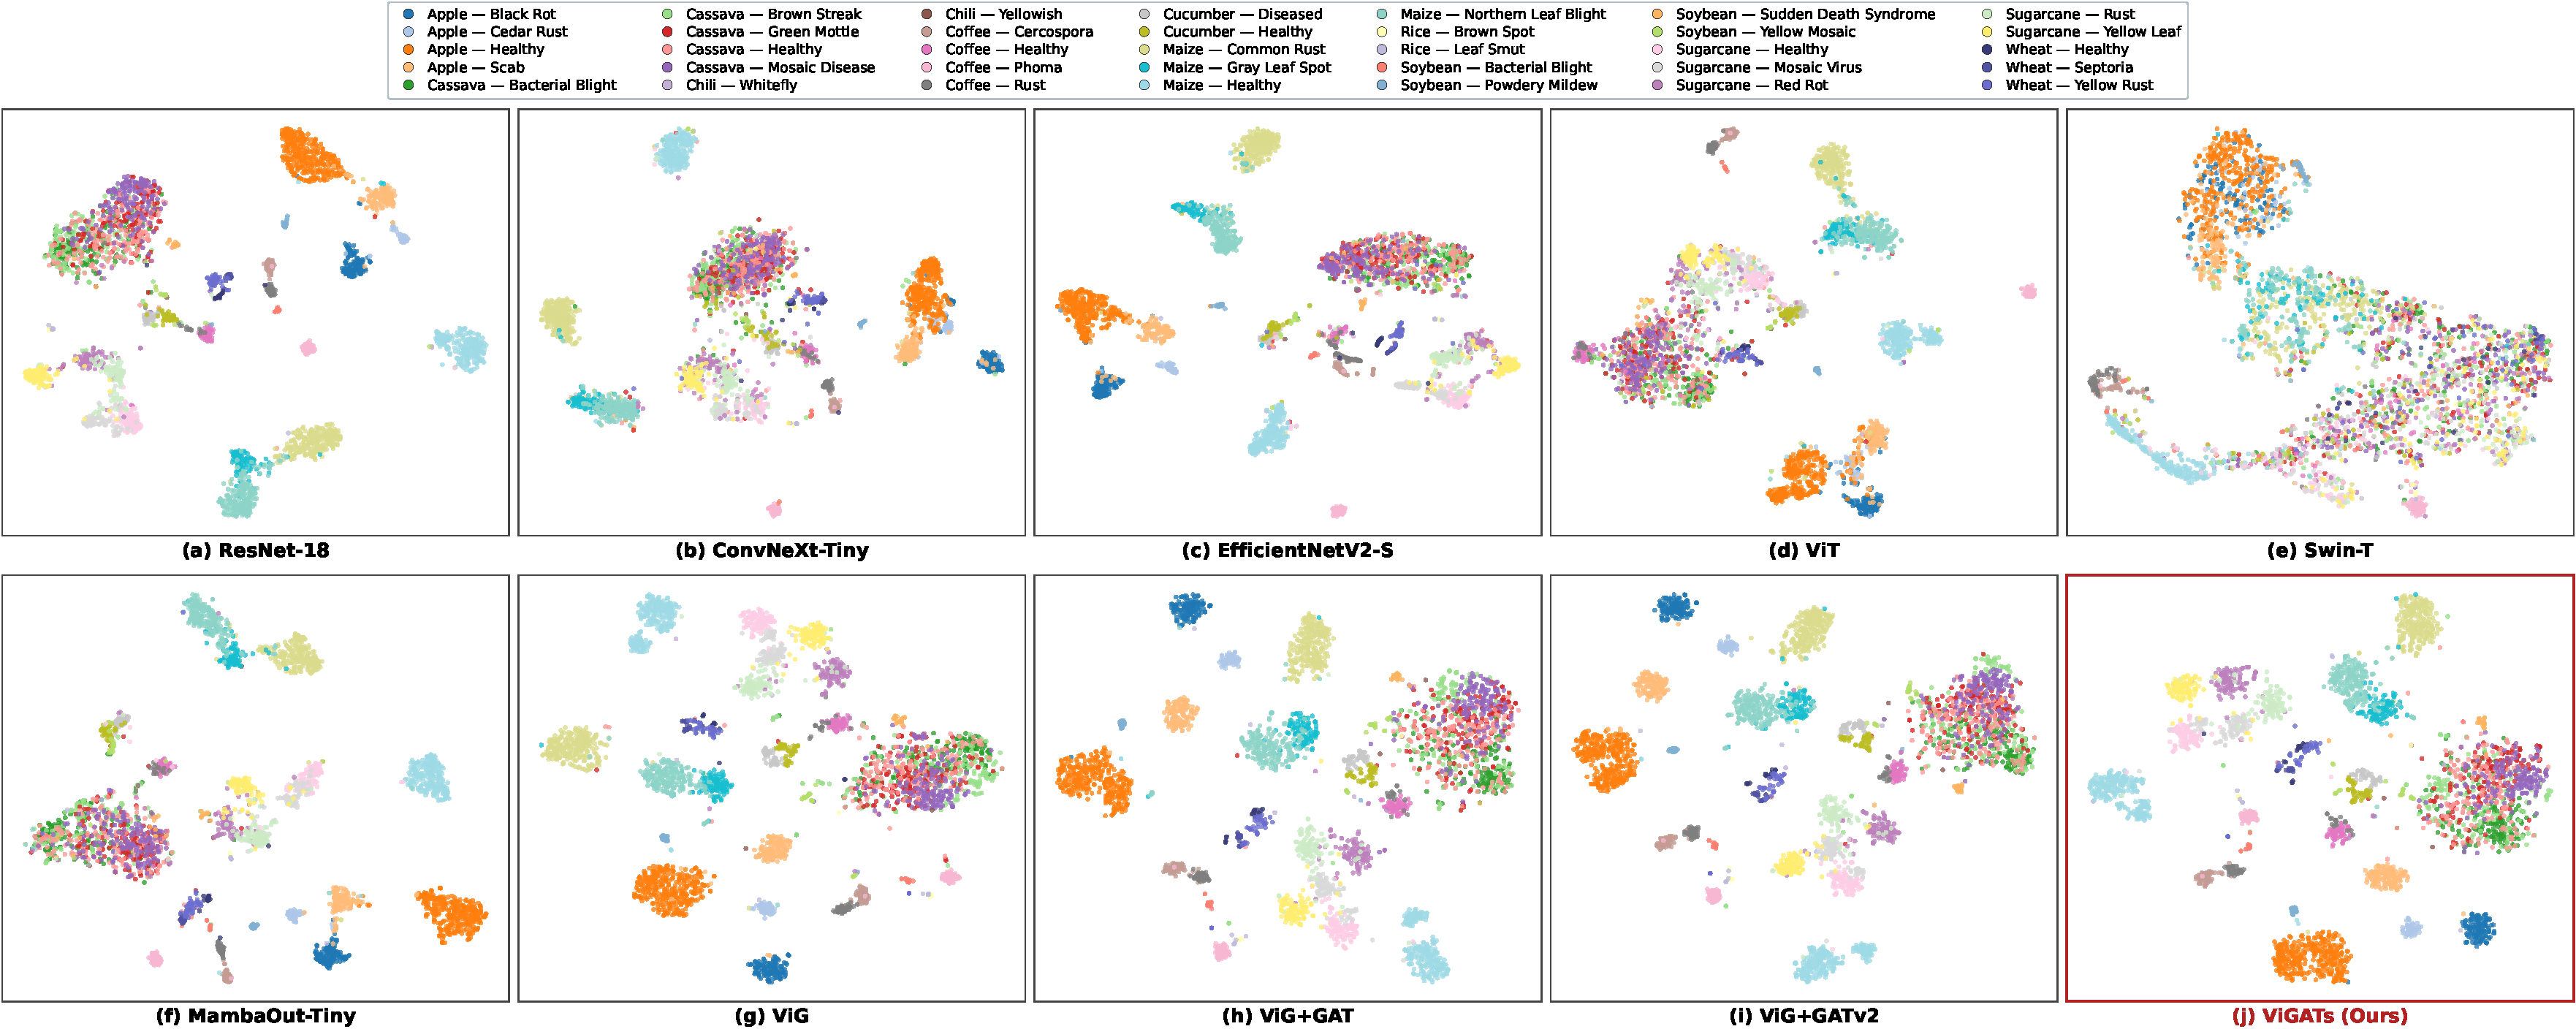
\includegraphics[width=\textwidth]{figures/Figure_08a_tsne_plantraw.pdf}%
\label{fig:tsne_plantraw}}

\vspace{3pt}
\subfloat[Rice Leaf Disease V2 (4 classes; 1,187 test images).]{%
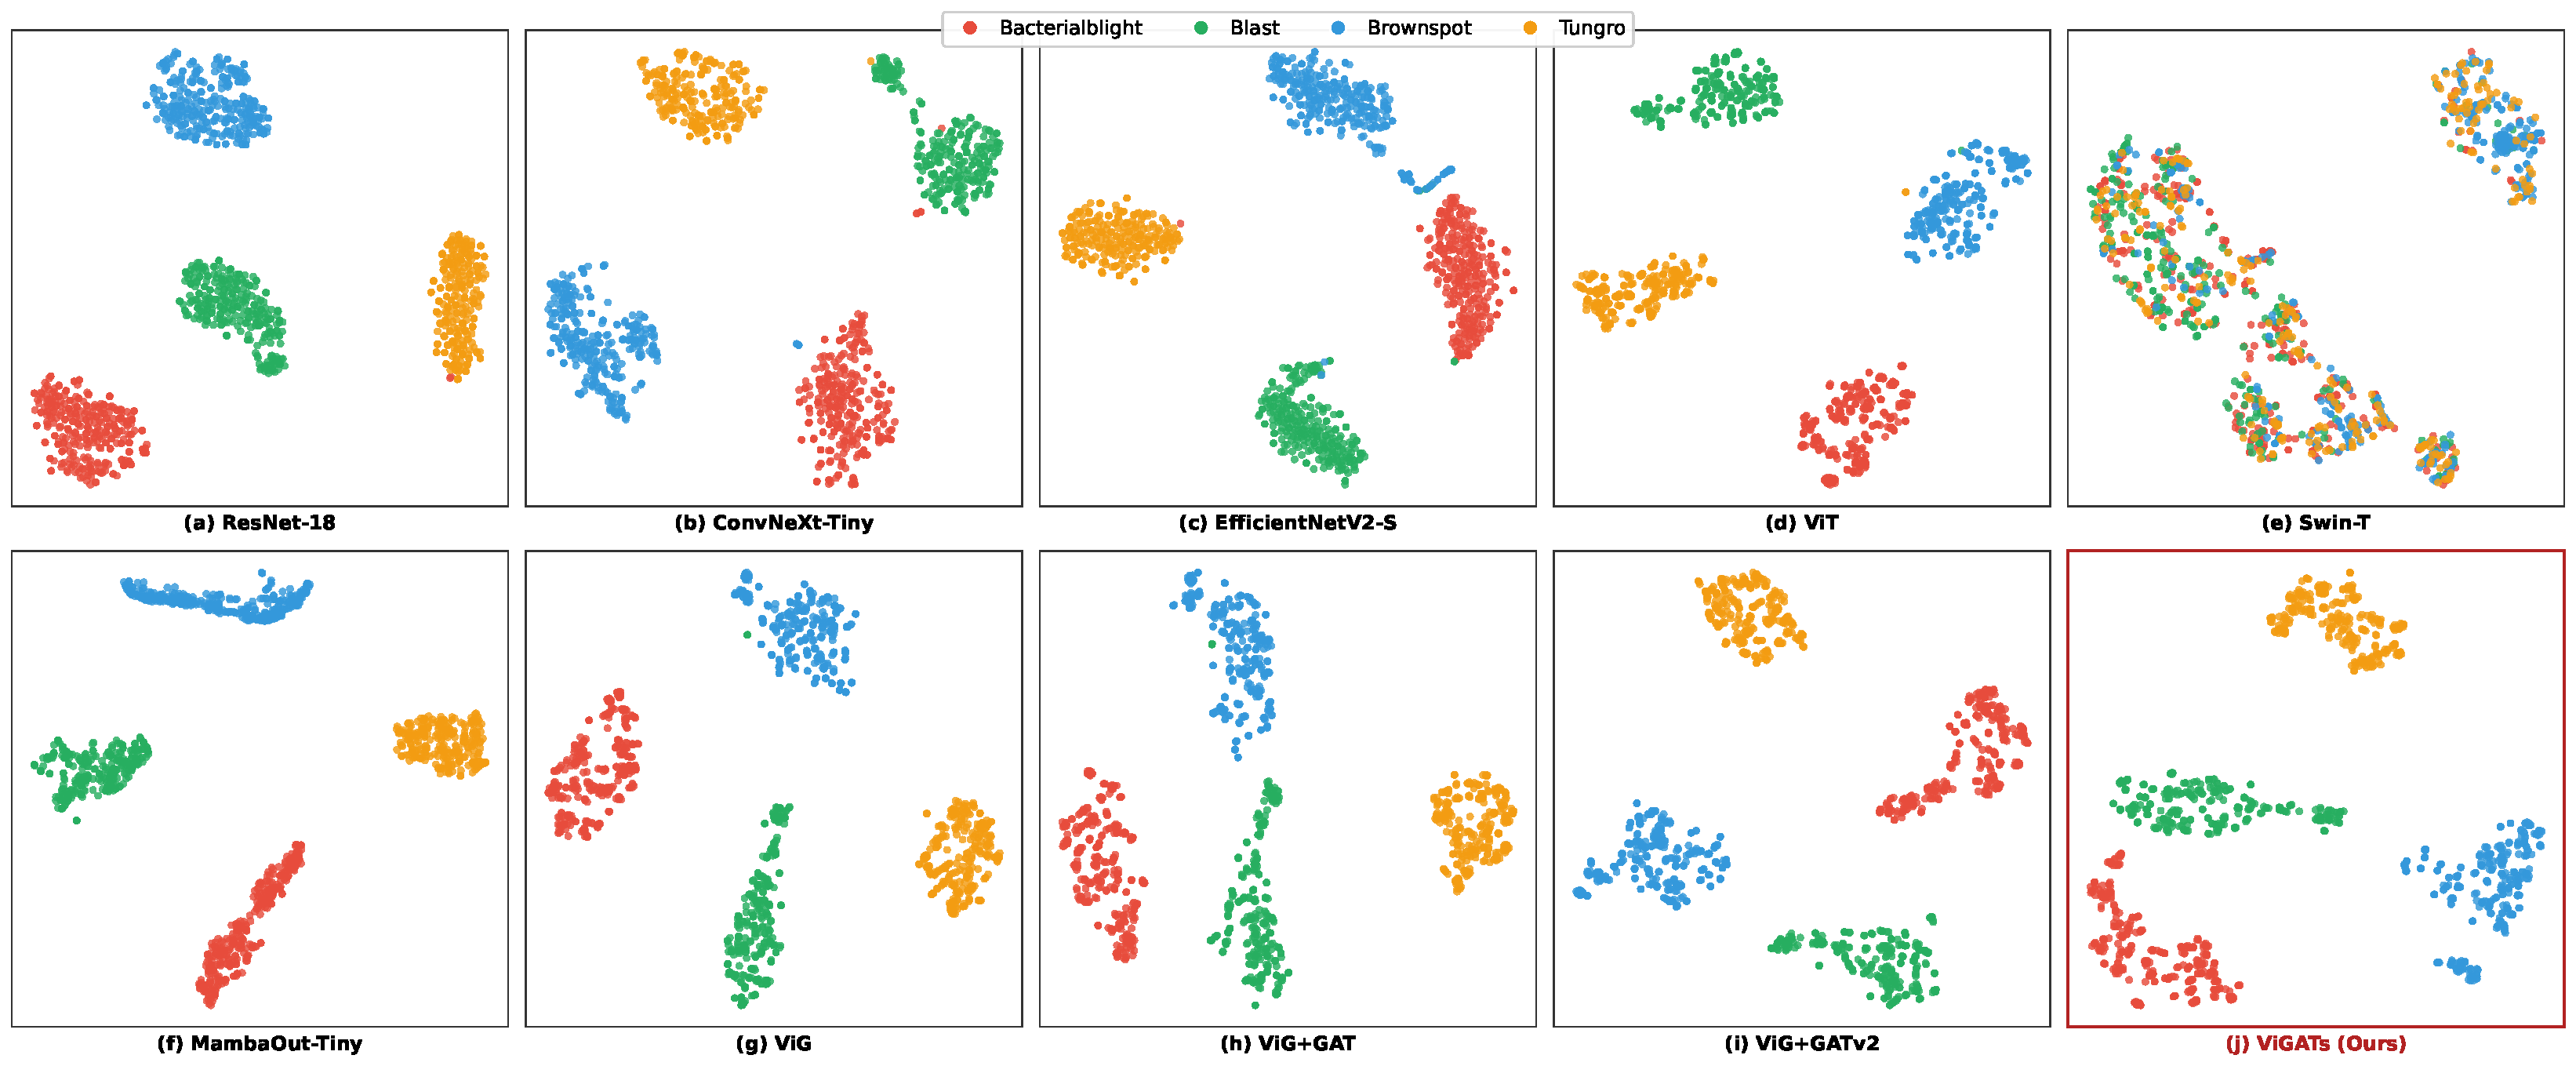
\includegraphics[width=\textwidth]{figures/Figure_08b_tsne_riceleaf.pdf}%
\label{fig:tsne_riceleaf}}
\caption{Qualitative t-SNE projections of fold-0 penultimate-layer features on (a) PlantRaw and (b) Rice Leaf Disease V2.}
\label{fig:tsne_combined}
\end{figure}


\section{Discussion and Explainability}
\label{sec:discussion}

\subsection{Efficacy of Edge-Difference Multi-Head Attention}
The superior generalization of ViGATs on natural field datasets (PlantRaw $86.12\%$ and Maize $98.58\%$) is directly attributed to the proposed GATConv operator:
\begin{itemize}
    \item \textit{Overcoming MRConv Bottlenecks:} Instead of rigid channel-wise max-pooling, GATConv dynamically learns soft attention weights over edge differences, adaptively magnifying pathological lesions while suppressing field background noise.
    \item \textit{Multi-Head Specialization ($H=4$):} Multi-head attention enables distinct heads to specialize in different morphological features (e.g., necrosis centers vs. chlorotic halos).
    \item \textit{Complexity vs. Accuracy Balance:} Grouped linear projections enable ViGATs to operate at only 1.13 GFLOPs and 4.67M parameters, providing an ideal computation profile for agricultural IoT devices.
\end{itemize}

\subsection{Visual Interpretability in Graph Feature Space}

\begin{figure}[H]
\centering
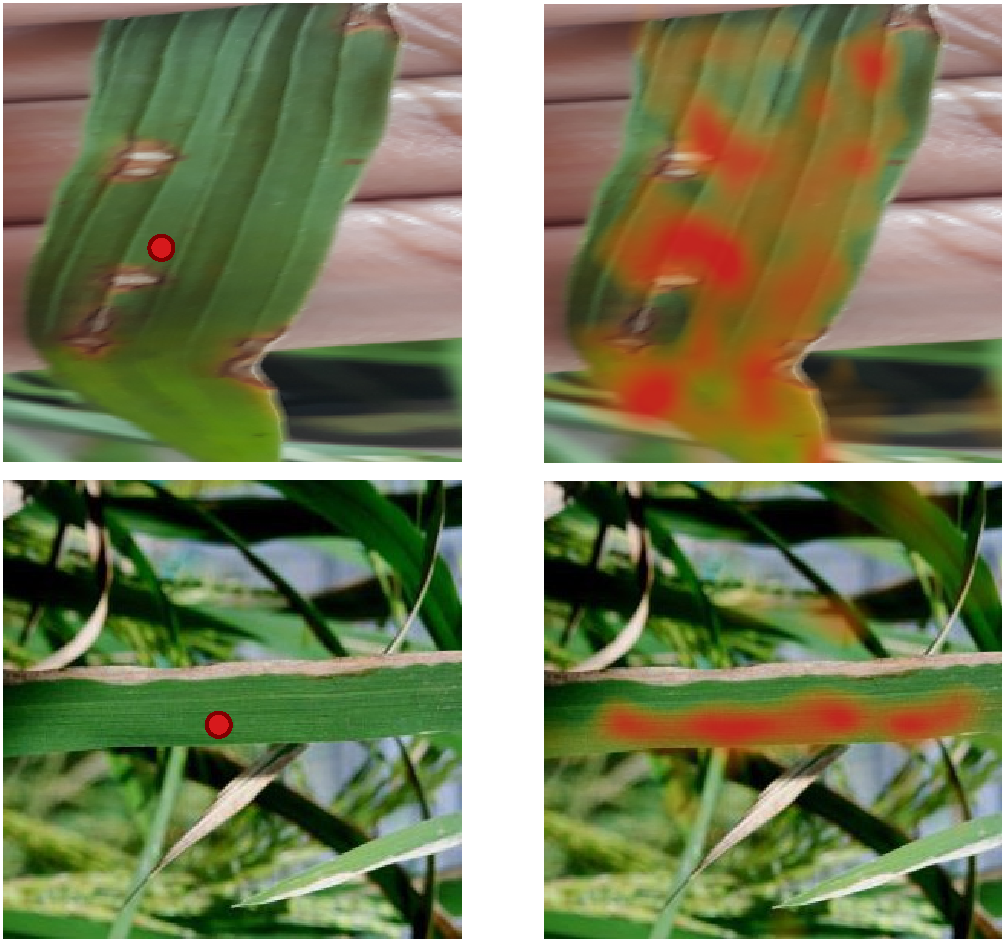
\includegraphics[width=0.82\textwidth]{figures/Figure_09_graph_neighborhood_riceleaf.pdf}
\caption{Query-key cosine-similarity visualization from Grapher block~1 of the ViGATs fold-4 checkpoint on Rice Blast (top) and Bacterial Blight (bottom).}
\label{fig:graph_neighborhood_riceleaf}
\end{figure}

Figure~\ref{fig:graph_neighborhood_riceleaf} visualizes query-key cosine similarities in Grapher block 1:
\begin{itemize}
    \item \textit{Non-Local Association (Top Row):} For a query lesion patch (red), the attention heatmap highlights disconnected lesion spots across the leaf, demonstrating that the dynamic $K$-NN graph captures semantic affinity beyond 2D Euclidean proximity.
    \item \textit{Lesion Stripe Delineation (Bottom Row):} Attention closely tracks linear bacterial blight lesions while sharply ignoring healthy leaf tissues and background clutter.
\end{itemize}

\subsection{Practical Deployment Potential and Limitations}
Operating at $64 \times 64$ resolution enables real-time edge processing on modest hardware platforms. While ViGATs achieves a throughput of 74 FPS on modern GPUs (suitable for drone and robotic video feeds), its inference latency is slightly higher than standard CNNs (such as ResNet-18) due to dynamic $K$-NN neighbor retrieval. Future optimizations exploring approximate nearest neighbor search and TensorRT engine compilation will further accelerate throughput.


\section{Conclusion}
\label{sec:conclusion}

This study presented ViGATs, an isotropic Vision Graph Attention Network engineered for robust botanical disease diagnosis. By substituting MRConv with the proposed GATConv module featuring multi-head edge-difference attention, ViGATs resolves the challenges of scattered pathological symptoms and complex natural background noise. Rigorous 5-fold stratified cross-validation across four diverse plant disease benchmarks ($96.09\%$ average accuracy), PlantRaw ($86.12\%$), and drone transfer scenarios demonstrates that ViGATs delivers state-of-the-art diagnostic accuracy with a compact model footprint (4.67M parameters, 1.13 GFLOPs), paving the way for efficient Edge AI deployment in smart agriculture.


\section*{Declarations}

\textit{Acknowledgement(s).} [Anonymized for Double-Blind Peer Review].

\textit{Disclosure statement.} The authors declare that they have no competing financial or non-financial interests to report.

\textit{Use of Generative AI in Writing.} Generative AI (Google Gemini) was employed during manuscript preparation exclusively for grammatical refinements, formatting assistance, and minor script debugging. The AI tool did not contribute to formulating scientific hypotheses, developing research methodologies, interpreting experimental data, or drawing conclusions; all academic concepts and final interpretations remain entirely the authors' own work.

\textit{Funding.} This research received no external funding.

\textit{Author contributions.} [Anonymized for Double-Blind Peer Review].

\textit{ORCID.} [Anonymized for Double-Blind Peer Review].

\textit{Data availability statement.} The datasets analyzed in this study are publicly available and properly cited. The complete PlantRaw dataset, metadata and standardized train/test splits are permanently archived on Zenodo \citep{tongle2026plantraw}: \url{https://doi.org/10.5281/zenodo.21869021}. The experimental logs and best pre-trained ViGATs weights are openly available at \url{https://github.com/tonglethanhhai/ViGATs_Results}.

\textit{Ethics statement.} This study did not involve human participants or animal experiments (Ethical Approval: Not applicable).

\bibliographystyle{tjit}
\begin{thebibliography}{99}

\bibitem[Atila et~al.(2021)]{atila2021plant}
Atila, \"{U}., U\c{c}ar, M., Akyol, K., \& U\c{c}ar, E. (2021). Plant leaf disease classification using EfficientNet deep learning model. \emph{Ecological Informatics}, \emph{61}, 101182.

\bibitem[Batool et~al.(2025)]{batool2025compact}
Batool, A., Kim, J., \& Byun, Y.-C. (2025). A compact deep learning approach integrating depthwise convolutions and spatial attention for plant disease classification. \emph{Plant Methods}, \emph{21}, Article~48. \url{https://doi.org/10.1186/s13007-025-01325-4}.

\bibitem[Borhani et~al.(2022)]{borhani2022deep}
Borhani, Y., Khoramdel, J., \& Najafi, E. (2022). A deep learning based approach for automated plant disease classification using vision transformer. \emph{Scientific Reports}, \emph{12}, 11554.

\bibitem[Brody et~al.(2022)]{brody2022gat}
Brody, S., Alon, U., \& Yahav, E. (2022). How attentive are graph attention networks? In \emph{Proc. ICLR}.

\bibitem[Cai et~al.(2023)]{cai2023efficientvit}
Cai, H., Li, J., Hu, M., Gan, C., \& Han, S. (2023). EfficientViT: Lightweight multi-scale attention for on-device semantic segmentation. In \emph{Proc. IEEE CVPR} (pp.~13783--13793).

\bibitem[Chen et~al.(2021)]{chen2021identification}
Chen, J., Zhang, D., Suzauddola, M., Nanehkaran, Y., \& Sun, Y. (2021). Identification of plant disease images via a squeeze-and-excitation MobileNet model and twice transfer learning. \emph{IET Image Processing}, \emph{15}(5), 1115--1127.

\bibitem[Daphal \& Koli(2022)]{daphal2022sugarcane}
Daphal, S., \& Koli, S. (2022). Sugarcane leaf disease dataset (Version~1) [Data set]. \emph{Mendeley Data}. \url{https://doi.org/10.17632/9424skmnrk.1}.

\bibitem[Dosovitskiy et~al.(2021)]{dosovitskiy2020image}
Dosovitskiy, A., Beyer, L., Kolesnikov, A., Weissenborn, D., Zhai, X., Unterthiner, T., Dehghani, M., Minderer, M., Heigold, G., Gelly, S., Uszkoreit, J., \& Houlsby, N. (2021). An image is worth 16x16 words: Transformers for image recognition at scale. In \emph{Proc. ICLR}.

\bibitem[Ferentinos(2018)]{ferentinos2018deep}
Ferentinos, K.~P. (2018). Deep learning models for plant disease detection and diagnosis. \emph{Computers and Electronics in Agriculture}, \emph{145}, 311--318.

\bibitem[Gedik et~al.(2025)]{gedik2025attentionvig}
Gedik, H. E., Martin, A., Munir, M., Baser, O., Marculescu, R., Chinchali, S. P., \& Bovik, A. C. (2025). AttentionViG: Cross-attention-based dynamic neighbor aggregation in Vision GNNs. \emph{arXiv preprint arXiv:2509.25570}.

\bibitem[Getch(2021)]{getch2021wheat}
Getch, O. (2021). Wheat leaf dataset [Data set]. \emph{Kaggle}. \url{https://www.kaggle.com/datasets/olyadgetch/wheat-leaf-dataset}.

\bibitem[Han et~al.(2022)]{han2022vision}
Han, K., Wang, Y., Guo, J., Tang, Y., \& Wu, E. (2022). Vision GNN: An image is worth graph of nodes. In \emph{Proc. NeurIPS} (pp.~8291--8303).

\bibitem[He et~al.(2016)]{he2016deep}
He, K., Zhang, X., Ren, S., \& Sun, J. (2016). Deep residual learning for image recognition. In \emph{Proc. IEEE CVPR} (pp.~770--778).

\bibitem[Hendrycks \& Gimpel(2016)]{hendrycks2016gaussian}
Hendrycks, D., \& Gimpel, K. (2016). Gaussian error linear units (GELUs). \emph{arXiv preprint arXiv:1606.08415}.

\bibitem[Hughes \& Salath\'{e}(2015)]{hughes2015plantvillage}
Hughes, D.~P., \& Salath\'{e}, M. (2015). An open access repository of images on plant health to enable the development of mobile disease diagnostics. \emph{arXiv preprint arXiv:1511.08060}.

\bibitem[Thakur et~al.(2024)]{iiitdmj2024dataset}
Thakur, P. S., Chaturvedi, S., Khanna, P., Sheorey, T., \& Ojha, A. (2024). IIITDMJ\_Maize [Data set]. \emph{IEEE DataPort}. \url{https://doi.org/10.21227/maize-2024}.

\bibitem[Ioffe \& Szegedy(2015)]{ioffe2015batch}
Ioffe, S., \& Szegedy, C. (2015). Batch normalization: Accelerating deep network training by reducing internal covariate shift. In \emph{Proc. ICML} (pp.~448--456).

\bibitem[Khiem et~al.(2026)]{khiem2026rebanet}
Khiem, N.~M., Huynh, T.~T., \& Quyen, N.~P. (2026). REBANet: A hybrid deep learning model for rice leaf disease prediction with Grad-CAM explainability. In \emph{Proc. ICCIES}, CCIS, Vol.~2943 (pp.~535--549). Springer.

\bibitem[Le \& Yang(2015)]{le2015tiny}
Le, Y., \& Yang, X. (2015). Tiny ImageNet visual recognition challenge. CS 231N Course Project, Stanford University.

\bibitem[LeCun et~al.(1998)]{lecun1998gradient}
LeCun, Y., Bottou, L., Bengio, Y., \& Haffner, P. (1998). Gradient-based learning applied to document recognition. \emph{Proceedings of the IEEE}, \emph{86}(11), 2278--2324.

\bibitem[LeCun et~al.(2015)]{lecun2015deep}
LeCun, Y., Bengio, Y., \& Hinton, G. (2015). Deep learning. \emph{Nature}, \emph{521}(7553), 436--444.

\bibitem[Li et~al.(2019)]{li2019deepgcns}
Li, G., M\"{u}ller, M., Thabet, A., \& Ghanem, B. (2019). DeepGCNs: Can GCNs go as deep as CNNs? In \emph{Proc. IEEE ICCV} (pp.~9267--9276).

\bibitem[Lin et~al.(2013)]{lin2013network}
Lin, M., Chen, Q., \& Yan, S. (2013). Network in network. In \emph{Proc. ICLR}.

\bibitem[Liu et~al.(2021)]{liu2021swin}
Liu, Z., Lin, Y., Cao, Y., Hu, H., Wei, Y., Zhang, Z., Lin, S., \& Guo, B. (2021). Swin Transformer: Hierarchical vision transformer using shifted windows. In \emph{Proc. IEEE ICCV} (pp.~10012--10022).

\bibitem[Liu et~al.(2022)]{liu2022convnext}
Liu, Z., Mao, H., Wu, C. Y., Feichtenhofer, C., Darrell, T., \& Xie, S. (2022). A ConvNet for the 2020s. In \emph{Proc. IEEE CVPR} (pp.~11976--11986).

\bibitem[Mduma \& Mayo(2023)]{mduma2023maize}
Mduma, N., \& Mayo, F. (2023). Maize imagery dataset---Tanzania (Version~1) [Data set]. \emph{Mendeley Data}. \url{https://doi.org/10.17632/fkw49mz3xs.1}.

\bibitem[Mishra(2023)]{mishra2023soybean}
Mishra, S. (2023). Soybean diseased leaf dataset [Data set]. \emph{Kaggle}. \url{https://www.kaggle.com/datasets/sivm205/soybean-diseased-leaf-dataset}.

\bibitem[Mohanty et~al.(2016)]{mohanty2016using}
Mohanty, S.~P., Hughes, D.~P., \& Salath\'{e}, M. (2016). Using deep learning for image-based plant disease detection. \emph{Frontiers in Plant Science}, \emph{7}, 1419.

\bibitem[Munir et~al.(2023)]{munir2023mobilevig}
Munir, M., Avery, W., \& Marculescu, R. (2023). MobileViG: Graph-based sparse attention for mobile vision applications. In \emph{Proc. IEEE/CVF CVPR Workshops} (pp.~2211--2219).

\bibitem[Mwebaze et~al.(2019)]{mwebaze2019icassava}
Mwebaze, E., Gebru, T., Frome, A., Nsumba, S., \& Tusubira, J. (2019). iCassava 2019 fine-grained visual categorization challenge. \emph{arXiv preprint arXiv:1908.02900}.

\bibitem[Nagarathna et~al.(2025)]{nagarathna2025intelligent}
Nagarathna, P., Haroon~P.~S., A.~L., Srinivasalu, G., \& Venkata, A.~K.~P. (2025). Intelligent plant disease detection and classification using HV-GNN with ontology-driven knowledge embedding. \emph{ITM Web of Conferences}, \emph{79}, 01047.

\bibitem[Negm(2021)]{negm2021cucumber}
Negm, K. (2021). Cucumber plant diseases dataset [Data set]. \emph{Kaggle}. \url{https://www.kaggle.com/datasets/kareem3egm/cucumber-plant-diseases-dataset}.

\bibitem[Prajapati et~al.(2017)]{prajapati2017rice}
Prajapati, H.~B., Shah, J.~P., \& Dabhi, V.~K. (2017). Detection and classification of rice plant diseases. \emph{Intelligent Decision Technologies}, \emph{11}(3), 357--373. \url{https://doi.org/10.3233/IDT-170301}.

\bibitem[Prakoso(2021)]{prakoso2021chili}
Prakoso, D.~D. (2021). Chili plant disease [Data set]. \emph{Kaggle}. \url{https://www.kaggle.com/datasets/dhenyd/chili-plant-disease}.

\bibitem[Sethy(2024)]{rice_dataset2022}
Sethy, P.~K. (2024). Rice leaf disease image samples (Version~2) [Data set]. \emph{Mendeley Data}. \url{https://doi.org/10.17632/fwcj7stb8r.2}.

\bibitem[Savary et~al.(2019)]{savary2019global}
Savary, S., Willocquet, L., Pethybridge, S. J., Esker, P., McRoberts, N., \& Nelson, A. (2019). The global burden of pathogens and pests on major food crops. \emph{Nature Ecology \& Evolution}, \emph{3}, 430--439.

\bibitem[Scarselli et~al.(2009)]{scarselli2009graph}
Scarselli, F., Gori, M., Tsoi, A.~C., Hagenbuchner, M., \& Monfardini, G. (2009). The graph neural network model. \emph{IEEE Transactions on Neural Networks}, \emph{20}(1), 61--80.

\bibitem[Sethy et~al.(2020)]{sethy2020deep}
Sethy, P.~K., Barpanda, N.~K., Rath, A.~K., \& Behera, S.~K. (2020). Deep feature based rice leaf disease identification using support vector machine. \emph{Computers and Electronics in Agriculture}, \emph{175}, 105527.

\bibitem[Singh et~al.(2020)]{singh2020plantdoc}
Singh, D., Jain, N., Jain, P., Kayal, P., Kumawat, S., \& Batra, N. (2020). PlantDoc: A dataset for visual plant disease detection in the wild. In \emph{Proc. ACM CoDS-COMAD} (pp.~249--253).

\bibitem[Singh et~al.(2024)]{singh2024comprehensive}
Singh, A., Sharma, R., \& Kumar, S. (2024). A comprehensive review of deep learning approaches for plant disease detection. \emph{Crop Science}, \emph{64}, 917--940.

\bibitem[Singla et~al.(2025)]{singla2025denseswingnnnet}
Singla, S., Gupta, A., \& Sharma, M. (2025). DenseSwinGNNNet: A novel deep learning framework for accurate turmeric leaf disease classification. \emph{Tech Science}.

\bibitem[Sokolova \& Lapalme(2009)]{sokolova2009systematic}
Sokolova, M., \& Lapalme, G. (2009). A systematic analysis of performance measures for classification tasks. \emph{Information Processing \& Management}, \emph{45}(4), 427--437.

\bibitem[Surekha \& Subha~Mastan~Rao(2026)]{surekha2026adjleafgnn}
Surekha, B., \& Subha~Mastan~Rao, T. (2026). AdjLeafGNN: A hybrid deep learning and graph neural network framework. \emph{Scientific Reports}, \emph{16}, Article~15629.

\bibitem[Tan \& Le(2019)]{tan2019efficientnet}
Tan, M., \& Le, Q. (2019). EfficientNet: Rethinking model scaling for convolutional neural networks. In \emph{Proc. ICML} (pp.~6105--6114).

\bibitem[Tan \& Le(2021)]{tan2021efficientnetv2}
Tan, M., \& Le, Q. (2021). EfficientNetV2: Smaller models and faster training. In \emph{Proc. ICML} (pp.~10096--10106).

\bibitem[Thakur et~al.(2023)]{thakur2022vision}
Thakur, P.~S., Sheorey, T., \& Ojha, A. (2023). VGG-ICNN: A lightweight CNN model for crop disease identification. \emph{Multimedia Tools and Applications}, \emph{82}, 497--520.

\bibitem[Tong-Le et~al.(2026)]{tongle2026plantraw}
Tong-Le, T.-H., Le, M.-H., \& Doan, T.-N. (2026). PlantRaw metadata: A multicrop plant disease benchmark for real-world generalization evaluation [Data set]. \emph{Zenodo}. \url{https://doi.org/10.5281/zenodo.21869021}.

\bibitem[Too et~al.(2019)]{too2019comparative}
Too, E.~C., Li, Y., Njuki, S., \& Liu, Y. (2019). A comparative study of fine-tuning deep learning models for plant disease identification. \emph{Computers and Electronics in Agriculture}, \emph{161}, 272--279.

\bibitem[Touvron et~al.(2021)]{touvron2021training}
Touvron, H., Cord, M., Douze, M., Massa, F., Sablayrolles, A., \& J\'{e}gou, H. (2021). Training data-efficient image transformers \& distillation through attention. In \emph{Proc. ICML}.

\bibitem[van der Maaten \& Hinton(2008)]{van2008visualizing}
van der Maaten, L., \& Hinton, G. (2008). Visualizing data using t-SNE. \emph{Journal of Machine Learning Research}, \emph{9}(11), 2579--2605.

\bibitem[Vasu et~al.(2023)]{vasu2023fastvit}
Anasosalu Vasu, P., Gabriel, J., Zhu, J., Tuzel, O., \& Ranjan, A. (2023). FastViT: A fast hybrid vision transformer using structural reparameterization. In \emph{Proc. IEEE ICCV}.

\bibitem[Vaswani et~al.(2017)]{vaswani2017attention}
Vaswani, A., Shazeer, N., Parmar, N., Uszkoreit, J., Jones, L., Gomez, A. N., Kaiser, \L., \& Polosukhin, I. (2017). Attention is all you need. In \emph{Proc. NeurIPS} (pp.~5998--6008).

\bibitem[Veli\v{c}kovi\'{c} et~al.(2018)]{velickovic2018graph}
Veli\v{c}kovi\'{c}, P., Cucurull, G., Casanova, A., Romero, A., Li\`{o}, P., \& Bengio, Y. (2018). Graph attention networks. In \emph{Proc. ICLR}.

\bibitem[Vo et~al.(2026)]{vo2026resnetkan}
Vo, H., Thien, N., Mui, K., Le, H., \& Tien, P. (2026). Enhanced tomato leaf disease diagnosis: A parameter-efficient approach using hybrid ResNet-KAN architectures. In \emph{Proc. ICCIES}, CCIS, Vol.~2943 (pp.~521--534). Springer.

\bibitem[Wang et~al.(2019)]{wang2019dynamic}
Wang, Y., Sun, Y., Liu, Z., Sarma, S. E., Bronstein, M. M., \& Solomon, J. M. (2019). Dynamic graph CNN for learning on point clouds. \emph{ACM Transactions on Graphics}, \emph{38}(5), 1--12.

\bibitem[Wang et~al.(2024)]{wang2024repvit}
Wang, A., Chen, H., Liu, L., Chen, K., Lin, Z., Han, J., \& Ding, G. (2024). RepViT: Revisiting mobile CNN from ViT perspective. In \emph{Proc. IEEE CVPR}.

\bibitem[Wu et~al.(2021)]{wu2020comprehensive}
Wu, Z., Pan, S., Chen, F., Long, G., Zhang, C., \& Yu, P. (2021). A comprehensive survey on graph neural networks. \emph{IEEE TNNLS}, \emph{32}(1), 4--24.

\bibitem[Yoseph(2023)]{yoseph2023coffee}
Yoseph, B. (2023). Ethiopian coffee leaf disease [Data set]. \emph{Kaggle}. \url{https://www.kaggle.com/datasets/biniyamyoseph/ethiopian-coffee-leaf-disease}.

\bibitem[Yu et~al.(2024)]{yu2024mambaout}
Yu, W. \& Wang, X. (2024). MambaOut: Do we really need Mamba for vision? \emph{arXiv preprint arXiv:2405.07992}.

\bibitem[Yu et~al.(2025)]{yu2025stcfi}
Yu, S., Xie, L., \& Dai, L. (2025). ST-CFI: Swin Transformer with convolutional feature interactions. \emph{Scientific Reports}, \emph{15}, Article~25000.

\bibitem[Zhang et~al.(2023)]{zhang2023dive}
Zhang, A., Lipton, Z. C., Li, M., \& Smola, A. J. (2023). \emph{Dive into deep learning}. Cambridge University Press.

\bibitem[Zhou et~al.(2020)]{zhou2020graph}
Zhou, J., Cui, G., Hu, S., Zhang, Z., Yang, C., Liu, Z., Wang, L., Li, C., \& Sun, M. (2020). Graph neural networks: A review of methods and applications. \emph{AI Open}, \emph{1}, 57--81.

\end{thebibliography}

\end{document}
